\documentclass[11pt,a4paper]{article}

% French
\usepackage[utf8x]{inputenc}
\usepackage[frenchb]{babel}
\usepackage[T1]{fontenc}
\usepackage{lmodern}
\usepackage{url}

% Math symbols
\usepackage{amsmath}
\usepackage{amssymb}
\usepackage{amsthm}
\usepackage{subfigure} %Allows to have several figures on the same line.
\usepackage{hyperref} %Allows to make references (\ref{}), pdf links are now clickable.
\usepackage{fmtcount} %Allows to use counters
\usepackage{fourier-orns} % Allows to display the \danger symbol

\usepackage{makeidx} %Allows to create an index
\usepackage{enumerate} %Used where??
\makeindex
\usepackage[totoc]{idxlayout} %Allows to add the index in the table of contents

% Theorem and definitions
\theoremstyle{definition}
\newtheorem{mydef}{Définition}[subsection]
\newtheorem{mynota}[mydef]{Notation}
\newtheorem{myprop}[mydef]{Propriétés}
\newtheorem{myrem}[mydef]{Remarque}
\newtheorem{myform}[mydef]{Formules}
\newtheorem{mycorr}[mydef]{Corrolaire}
\newtheorem{mytheo}[mydef]{Théorème}
\newtheorem{mylem}[mydef]{Lemme}
\newtheorem{myexem}[mydef]{Exemple}
\newtheorem{myalgo}[mydef]{Algorithme}

\newcommand{\bigoh}{\mathcal{O}}

\usepackage{tkz-graph}
\usepackage{tikz}
\usetikzlibrary{arrows,matrix,decorations.pathreplacing,positioning,chains,fit,shapes,calc} %Voir 1.3.8

\definecolor{mygreen}{rgb}{0,0.6,0}
\definecolor{mygray}{rgb}{0.5,0.5,0.5}
\definecolor{mymauve}{rgb}{0.58,0,0.82}

\tikzstyle{vertex}=[circle,fill=gray!50,minimum size=15pt,inner sep=0pt]
\tikzstyle{visited}=[circle,fill=green!25,minimum size=15pt,inner sep=0pt]
\tikzstyle{unvisited}=[circle,fill=blue!25,minimum size=15pt,inner sep=0pt]

\newcommand{\W}{\ {\color{red} \textbf{!!}} \ }

% Flots
\newcommand{\flotmax}{f_\mathrm{max}}
\DeclareMathOperator{\fnet}{f_\mathrm{net}}
\DeclareMathOperator{\coupe}{coupe}
\DeclareMathOperator{\degin}{\deg_\mathrm{in}}
\DeclareMathOperator{\degout}{\deg_\mathrm{out}}
\DeclareMathOperator{\valeur}{valeur}


\usepackage[framemethod=tikz]{mdframed}
%\usepackage{tikzpagenodes}
\usepackage{hyperref} %Allows to make references (\ref{}), pdf links are now clickable.
\usetikzlibrary{calc}

%http://tex.stackexchange.com/questions/107191/indented-box-that-split-in-multiple-pages
\mdfdefinestyle{mysquare}{%
  leftmargin=0pt,
  rightmargin={\dimexpr4pt+2ex\relax},
  innertopmargin=2\baselineskip,
  skipabove={\dimexpr0.5\baselineskip+\topskip\relax},
  skipbelow={\dimexpr0.5\baselineskip+\topskip\relax},
  singleextra={% Single extra applies when it fits in a single page
  \path let \p1=(P), \p2=(O)
    in node[font=\bfseries] at ([yshift=-2ex]0.5*\x1-\x2,\y1) {Solution};
  \fill[black] ([xshift=2pt,yshift=2pt]P) rectangle ++(1ex,1ex);
  \fill[black] ([xshift=-2pt,yshift=-2pt]O) rectangle ++(-1ex,-1ex);
  \fill[black] ([xshift=-2pt,yshift=2pt]O|-P) rectangle ++(-1ex,1ex);
  \fill[black] ([xshift=2pt,yshift=-2pt]O-|P) rectangle ++(1ex,-1ex);
  },
  firstextra={% First extra applies on the first page when it doesn't fit in one page
  \path let \p1=(P), \p2=(O)
    in node[font=\bfseries] at ([yshift=-2ex]0.5*\x1-\x2,\y1) {Solution};
  \fill[fill=black] ([xshift=2pt,yshift=2pt]P) rectangle ++(1ex,1ex);
  \fill[black] ([xshift=-2pt,yshift=2pt]O|-P) rectangle ++(-1ex,1ex);
  },
  secondextra={% First extra applies on the last page when it doesn't fit in one page
  \fill[fill=black] ([xshift=2pt,yshift=-2pt]O-|P) rectangle ++(1ex,-1ex);
  \fill[black] ([xshift=-2pt,yshift=-2pt]O) rectangle ++(-1ex,-1ex);
  }
}
\newmdenv[style=mysquare]{solution}

\newcommand{\nosolution}
{Cet exercice ne contient pas encore de solution.
Vous êtes invité à nous en soumettre une à l'adresse suivante
\begin{center}
\url{https://github.com/blegat/LINMA1702-exercices}
\end{center}
ou par mail.}

\parindent0mm

\setlength{\textwidth}{15cm}
\setlength{\oddsidemargin}{0.50cm}
\setlength{\textheight}{8.7in}
\setlength{\topmargin}{-0.5in}

\newcommand{\R}{{\mbox{\bf R}}}

\author{}

\title{INMA1691 - Théorie et Algorithmique des Graphes : Exercices}

\begin{document}
%%%%%%%%%%%%%%%%%%%%%%%%%%%%%%%%%%%%%%%%%%%%%%%%%%%%%%%%%%%%%%%
%%%%%%%%%%%%%%%%%%%%%%%% PAGE DE GARDE %%%%%%%%%%%%%%%%%%%%%%%%
%%%%%%%%%%%%%%%%%%%%%%%%%%%%%%%%%%%%%%%%%%%%%%%%%%%%%%%%%%%%%%%
\pagenumbering{gobble}% Remove page numbers
\maketitle
\begin{center}
  \textbf{Code source et bug tracker}\\
  \url{https://github.com/blegat/LINMA1691-exercices}\\
  \includegraphics[width=140pt]{../img/logo}
\end{center}
\newpage
\clearpage

%%%%%%%%%%%%%%%%%%%%%%%%%%%%%%%%%%%%%%%%%%%%%%%%%%%%%%%%%%%%%%%
%%%%%%%%%%%%%%%%%%%%%%% Table Of Contents %%%%%%%%%%%%%%%%%%%%%
%%%%%%%%%%%%%%%%%%%%%%%%%%%%%%%%%%%%%%%%%%%%%%%%%%%%%%%%%%%%%%%
\pagenumbering{arabic}% Arabic page numbers (and reset to 1)
\tableofcontents
\newpage

\section{Graphes connexes, eulériens et bipartis }
\subsection{Graphes}

\index{graphe}
\begin{mydef}
  Un \emph{graphe} est un triplet ($V$, $E$, $\varphi$), où :\\
  - $V$ est un ensemble dont les éléments sont appelés sommets ou noeuds; \\
  - $E$ est un ensemble dont les éléments sont appelés arêtes; \\
  - $\varphi$ est une fonction, dîte fonction d'incidence, qui associe à chaque arête un sommet ou une paire de sommets.
\end{mydef}

\index{sommets adjacents}
\begin{mydef}
  Deux sommets incidents à la même arête sont dits \emph{adjacents}.
\end{mydef}

\index{boucle}
\begin{mydef}
  Une arête incidente à un seul sommet est une \emph{boucle}.
\end{mydef}

\index{degré}
\begin{mydef}
  Le \emph{degré} d'un sommet est le nombre d'arêtes incidentes à celui-ci.
\end{mydef}

\index{graphe!sous-graphe}
\begin{mydef}
  Un \emph{sous-graphe du graphe} ($V$, $E$, $\varphi$) est un graphe ($V'$, $E'$, $\varphi'$) avec : \\
  - $V' \subseteq V$ ; \\
  - $E' \subseteq E$ ; \\
  - $\varphi'$ est la restriction de $\varphi'$ à $E'$.
\end{mydef}

\index{isomorphisme}
\subsection{Isomorphisme de Graphes}
\begin{mydef}
  Deux graphes ($V$, $E$, $\varphi$) et ($V'$, $E'$, $\varphi'$) sont dits \emph{isomorphes} s'il existe des bijections $f:V \to V'$ et $g:E \to E'$ telles que :
  \begin{center}
    $\varphi(e) = \{u, v\}$ ssi $\varphi(g(e)) = \{f(u), f(v)\}$.
  \end{center}
  Deux graphes sont isomorphes s'il y a une bijection entre les noeuds et les arêtes.
\end{mydef}

\begin{myexem}
  Voici deux exemples d'isomorphisme du même graphe :
    \begin{figure} [!h]
      \centering
	    \subfigure[]
    	{
    	  \begin{tikzpicture}[scale = 0.75]
          \node[draw, circle] at ( 0, 1.5)  (1) {1};
          \node[draw, circle] at ( 2, 0  )  (2) {2};
          \node[draw, circle] at ( 1,-1.5)  (3) {3};
          \node[draw, circle] at (-1,-1.5)  (4) {4};
          \node[draw, circle] at (-2, 0  )  (5) {5};

          \draw[-] (1) edge [bend left] node[anchor = south] {a} (2);
          \draw[-] (2) edge [bend left] node[anchor = west]  {b} (3);
          \draw[-] (3) edge [bend left] node[anchor = north] {c} (4);
          \draw[-] (4) edge [bend left] node[anchor = east]  {d} (5);
          \draw[-] (5) edge [bend left] node[anchor = east]  {e} (1);
        \end{tikzpicture}
      }
      % Cette ligne de commentaire semble être nécessaire pour que les figures soient affichées sur une ligne
      \subfigure[]
      {
        \begin{tikzpicture}[scale = 0.75]
          \node[draw, circle] at ( 0, 1.5)  (1) {$1'$};
          \node[draw, circle] at ( 2, 0  )  (2) {$2'$};
          \node[draw, circle] at ( 1,-1.5)  (3) {$3'$};
          \node[draw, circle] at (-1,-1.5)  (4) {$4'$};
          \node[draw, circle] at (-2, 0  )  (5) {$5'$};

          \draw[-] (1) edge node {$a'$} (3); %TODO mettre le label autrement pour que ce soit lisible
          \draw[-] (2) edge node {$b'$} (5); %TODO mettre le label autrement pour que ce soit lisible
          \draw[-] (2) edge node {$c'$} (4); %TODO mettre le label autrement pour que ce soit lisible
          \draw[-] (3) edge node {$d'$} (5); %TODO mettre le label autrement pour que ce soit lisible
          \draw[-] (1) edge node {$e'$} (4); %TODO mettre le label autrement pour que ce soit lisible

          %TODO tracer les lignes qui montrent comment on passe du graphe b au graphe c (en gardant les 3 graphes sur la même ligne)

        \end{tikzpicture}
      }
      % Cette ligne de commentaire semble être nécessaire pour que les figures soient affichées sur une ligne
      \subfigure[]
      {
        \begin{tikzpicture}[scale = 0.75]
          \node[draw, circle] at ( 0, 1.5)  (1) {$1'$};
          \node[draw, circle] at ( 2, 0  )  (4) {$4'$};
          \node[draw, circle] at ( 1,-1.5)  (2) {$2'$};
          \node[draw, circle] at (-1,-1.5)  (5) {$5'$};
          \node[draw, circle] at (-2, 0  )  (3) {$3'$};

          \draw[-] (1) edge [bend left] node[anchor = south] {$e'$} (4);
          \draw[-] (4) edge [bend left] node[anchor = west]  {$c'$} (2);
          \draw[-] (2) edge [bend left] node[anchor = north] {$b'$} (5);
          \draw[-] (5) edge [bend left] node[anchor = east]  {$d'$} (3);
          \draw[-] (3) edge [bend left] node[anchor = east]  {$a'$} (1);
        \end{tikzpicture}
      }
    \end{figure}
    Notons que les graphes \emph{b} et \emph{c} sont les mêmes, leurs noeuds ont simplement été réordonnés.\\
    L'isomorphisme entre \emph{a} et les deux autres est donné par : \\

    \begin{tabular}{lll}
      $f(1)=1'$ & $g(a)=e'$ \\
      $f(2)=4'$ & $g(b)=c'$ & $\varphi(a) = \{1, 2\}$\\
      $f(3)=2'$ & $g(c)=b'$ & $\varphi'(a') = \{1', 3'\}$\\
      $f(4)=5'$ & $g(d)=d'$ & $\varphi'(g(a)) = \{f(1), f(2)\}$\\
      $f(5)=3'$ & $g(e)=a'$ \\
    \end{tabular}
    \newline
    \newline
    Notons aussi que plusieurs résultats sont possibles : \\
    \begin{figure}[!h]
      \centering
      \subfigure[]
      {
        \begin{tikzpicture}[scale = 0.75]
          \node[draw, circle] at ( 0, 1.5)  (1) {1};
          \node[draw, circle] at ( 2, 0  )  (2) {2};
          \node[draw, circle] at ( 1,-1.5)  (3) {3};
          \node[draw, circle] at (-1,-1.5)  (4) {4};
          \node[draw, circle] at (-2, 0  )  (5) {5};

          \draw[-] (1) edge [bend left] node[anchor = south] {a} (2);
          \draw[-] (2) edge [bend left] node[anchor = west]  {b} (3);
          \draw[-] (3) edge [bend left] node[anchor = north] {c} (4);
          \draw[-] (4) edge [bend left] node[anchor = east]  {d} (5);
          \draw[-] (5) edge [bend left] node[anchor = east]  {e} (1);
        \end{tikzpicture}
      }
      % Cette ligne de commentaire semble être nécessaire pour que les figures soient affichées sur une ligne
      \subfigure[]
      {
        \begin{tikzpicture}[scale = 0.75]
          \node[draw, circle] at ( 0, 1.5)  (1) {$1'$};
          \node[draw, circle] at ( 2, 0  )  (2) {$2'$};
          \node[draw, circle] at ( 1,-1.5)  (3) {$3'$};
          \node[draw, circle] at (-1,-1.5)  (4) {$4'$};
          \node[draw, circle] at (-2, 0  )  (5) {$5'$};

          \draw[-] (1) edge node {$a'$} (3); %TODO mettre le label autrement pour que ce soit lisible
          \draw[-] (2) edge node {$b'$} (5); %TODO mettre le label autrement pour que ce soit lisible
          \draw[-] (2) edge node {$c'$} (4); %TODO mettre le label autrement pour que ce soit lisible
          \draw[-] (3) edge node {$d'$} (5); %TODO mettre le label autrement pour que ce soit lisible
          \draw[-] (1) edge node {$e'$} (4); %TODO mettre le label autrement pour que ce soit lisible

          %TODO tracer les lignes qui montrent comment on passe du graphe e au graphe f (en gardant les 3 graphes sur la même ligne)
        \end{tikzpicture}
      }
      % Cette ligne de commentaire semble être nécessaire pour que les figures soient affichées sur une ligne
      \subfigure[]
      {
        \begin{tikzpicture}[scale = 0.75]
          \node[draw, circle] at ( 0, 1.5)  (1) {$1'$};
          \node[draw, circle] at ( 2, 0  )  (3) {$3'$};
          \node[draw, circle] at ( 1,-1.5)  (5) {$5'$};
          \node[draw, circle] at (-1,-1.5)  (2) {$2'$};
          \node[draw, circle] at (-2, 0  )  (4) {$4'$};

          \draw[-] (1) edge [bend left] node[anchor = south] {$a'$} (3);
          \draw[-] (3) edge [bend left] node[anchor = west]  {$d'$} (5);
          \draw[-] (5) edge [bend left] node[anchor = north] {$b'$} (2);
          \draw[-] (2) edge [bend left] node[anchor = east]  {$c'$} (4);
          \draw[-] (4) edge [bend left] node[anchor = east]  {$e'$} (1);
        \end{tikzpicture}
      }
    \end{figure}

    \begin{tabular}{lll}
      $f(1)=1'$ & $g(a)=a'$ \\
      $f(2)=3'$ & $g(b)=b'$ \\
      $f(3)=5'$ & $g(c)=d'$ \\
      $f(4)=2'$ & $g(d)=c'$ \\
      $f(5)=4'$ & $g(e)=e'$ \\
    \end{tabular}
    \newline
    \newline
    Les six graphes de cet exemple sont isomorphes entre eux.
\end{myexem}

\subsection{Parcours eulérien}
\index{parcours}
\begin{mydef}%TODO définir ce qu'est un parcours
  Un \emph{parcours} est fermé si $v_0 = v_1$.
\end{mydef}

\index{chemin}
\begin{mydef}
  Un \emph{chemin} est un parcours dont tous les sommets sont distincts.
\end{mydef}

\index{cycle}
\begin{mydef}
  Un \emph{cycle} est un parcours fermé dont tous les sommets d'origine et intérieurs sont tous distincts.
\end{mydef}

\index{graphe!graphe connexe}
\begin{mydef}
  Un \emph{graphe} est \emph{connexe} si pour chaque pair de points il existe un parcours qui les relie. Les \emph{composantes connexes} d'un graphe sont ses sous-graphes connexes maximaux.
\end{mydef}

\index{parcours!parcours eulérien}
\index{graphe!graphe eulérien}
\begin{mydef}
  Un \emph{parcours} est \emph{eulérien} s'il visite chaque arête une et une seule fois. Un \emph{graphe} est \emph{eulérien} s'il existe un parcours eulérien fermé.
\end{mydef}

\begin{mytheo} [Théorème d'Euler]
  Un graphe connexe est eulérien ssi tous les sommets sont de degré pair.
  \begin{proof}
    \noindent
    \newline
    \fbox{$\Longrightarrow$}
    \newline
    Chaque arête incidente à un noeud $x$ est utilisé par le parcours eulérien:
    \begin{itemize}
      \item soit pour entrer dans $x$;
      \item soit pour en sortir.\\
    \end{itemize}
    A chaque arête entrante correspond une arête sortante (celle qui suit dans le parcours sauf pour la dernière et la première).\\
    Donc, il y a une bijection entre les arêtes entrantes et les arêtes sortantes.\\
    $\longrightarrow$ degré pair \\

    \noindent
    \fbox{$\Longleftarrow$}
    \newline
    On va construire un parcours un parcours eulérien :\\
    \begin{enumerate}
      \item On part d'un noeud arbitraire $x_0$.
      \item On prend une arête incidente à $x_0$, on arrive à un nouveau noeud.
      \item Par parité, il y a au moins une arête non utilisée, on la prend, etc... Quand il n'y a plus d'arête disponible, on est forcément arrivé à $x_0$.\\
    \end{enumerate}

    INSERT GRAPH HERE \href{https://dl.dropboxusercontent.com/u/44092863/Graph_Theory_Romain_Capron.pdf}{Voir notes} \addTODO\\

    Pour tout autre noeud y, en arrivant à y, on a utilisé un nombre impair d'arêtes incidentes à y. On a un parcours fermé :
    \begin{itemize}
      \item Si toutes les arêtes incidentes aux x noeuds traversés par ce parcours sont utilisées, alors ce parcours est eulérien;
      \item Sinon, il y a $x_1 \in$ parcours avec au moins une arête non exploitée.\\
    \end{itemize}

    INSERT GRAPH HERE \href{https://dl.dropboxusercontent.com/u/44092863/Graph_Theory_Romain_Capron.pdf}{Voir notes} \addTODO\\

    On merge les deux parcours :\\
    $P_{0+1} = x_0 \rightarrow x_1 \textcolor{red}{\rightarrow} x_1 \rightarrow x_0$\\
    Et on fait ça en boucle jusqu'à avoir toutes les arêtes.
  \end{proof}
\end{mytheo}

\begin{mytheo} [Existence d’un parcours eulérien]
  Un graphe connexe possède un parcours eulérien ssi le nombre de noeuds de degré impair est zéro ou deux.
  \begin{proof} In Progress
    \noindent
    \newline
    \fbox{$\Longrightarrow$}
    \newline
    \begin{itemize}
      \item ;
      \item .\\
    \end{itemize}

    \noindent
    \fbox{$\Longleftarrow$}
    \newline
  \end{proof}
\end{mytheo}

\begin{mytheo} [Théorème des poignées de mains]
  La somme des degrés des noeuds d’un graphe est deux fois le nombre d’arêtes.
  \begin{proof}
     \href{https://dl.dropboxusercontent.com/u/44092863/Graph_Theory_Romain_Capron.pdf}{Voir notes} \addTODO
  \end{proof}
\end{mytheo}

\subsection{Représentation matricielle du graphe}
\index{matrice d'adjacence}
\begin{mydef}
  La \emph{matrice d'adjacence} est une matrice carrée $n$x$n$ dont l'élément $ij$ est le nombre d'arêtes entre les sommets $v_i$ et $v_j$.
\end{mydef}

\index{matrice d'incidence}
\begin{mydef}
  La \emph{matrice d'incidence} est une matrice rectangulaire $n$x$m$ dont l'élément $ij$ est le nombre de fois que le sommet $v_i$ est incident à l'arête $e_j$.
\end{mydef}

\begin{myexem}
  \href{https://dl.dropboxusercontent.com/u/44092863/Graph_Theory_Romain_Capron.pdf}{Voir notes} \addTODO
\end{myexem}

\begin{mytheo} [Matrice d’adjacence et nombre de parcours]
  Soit $A$ la matrice d'adjacence d'un graphe. Alors l'élément $ij$ de $A^k$ ($k \geq 0$) est le nombre de parcours de longueur $k$ de $v_i$ vers $v_j$.
  \begin{proof}
     \href{https://dl.dropboxusercontent.com/u/44092863/Graph_Theory_Romain_Capron.pdf}{Voir notes} \addTODO
  \end{proof}
\end{mytheo}

\index{distance entre deux noeuds}
\begin{mydef}
  La \emph{distance $d(u, v)$} entre les noeuds $u$ et $v$ d'un graphe est le nombre d'arêtes minimal d'un parcours entre ces deux noeuds.
\end{mydef}

\begin{mylem}
  Si $u...u'...v'...v$ est un parcours de longeur minimale de $u$ vers $v$, alors le sous-parcours $u'...v'$ est un parcours de longeur minimale de $u'$ vers $v'$.\\
  En particulier, un parcours de longueur minimale est toujours un chemin.
  \begin{proof}
    Si ce parcours entre $u'$ et $v'$ n'était pas le plus court, on utiliserait le parcours strictement plus court pour la construction du parcours entre $u$ et $v$.
  \end{proof}
\end{mylem}

\subsection{Graphe biparti}
\index{graphe!graphe biparti}
\begin{mydef}
  Un graphe est \emph{biparti}  s'il existe une partition en deux ensembles $V_1$ et $V_2$ tels que les sommets de $V_1$ ne sont adjacents qu'à des sommets de $V_2$ et vice versa. La bipartition est $(V_1, V_2)$.
\end{mydef}

\begin{myexem}
  \href{https://dl.dropboxusercontent.com/u/44092863/Graph_Theory_Romain_Capron.pdf}{Voir notes} \addTODO
\end{myexem}

\begin{mytheo} [Graphes bipartis]
  Un graphe est biparti ssi tous ses cycles sont de longueur paire.
  \begin{proof}
     \href{https://dl.dropboxusercontent.com/u/44092863/Graph_Theory_Romain_Capron.pdf}{Voir notes} \addTODO
  \end{proof}
\end{mytheo}

\section{Séance 2}
\paragraph{1. } Dans le graphe ci-dessous, trouvez le nombre de parcours fermés contenant le point $A$.

\begin{figure}[h!]
  \begin{center}
    \begin{tikzpicture}[scale=1,looseness=1,auto,line width=.4mm]

      \path[draw=none] (-2.3,1.3) node { $A$ };

      \draw (-2, 1) -- ( 0,-1);
      \draw (-2, 1) -- ( 2,-1);
      \draw ( 0, 1) -- (-2,-1);
      \draw ( 0, 1) -- ( 2,-1);
      \draw ( 2, 1) -- (-2,-1);
      \draw ( 2, 1) -- ( 0,-1);

      \draw[fill=black] (-2,-1) circle(.12);
      \draw[fill=black] (-2, 1) circle(.12);
      \draw[fill=black] ( 0,-1) circle(.12);
      \draw[fill=black] ( 0, 1) circle(.12);
      \draw[fill=black] ( 2,-1) circle(.12);
      \draw[fill=black] ( 2, 1) circle(.12);

    \end{tikzpicture}
  \end{center}
\end{figure}

On cherche le nombre de parcours fermé partant de A de longueur $k$.
Pour cela, on utilise le théorème suivant :

$\,$

Soit $A$ la matrice d'adjacence d'un graphe. Alors l'élément $ij$
de $A^{k}$ ($k\geq0$) est le nombre de parcours de longueur $k$
de $v_{i}$ vers $v_{j}$.

$\,$

Dans notre cas, le graphe est biparti non complet et la matrice d'adjacence
est donnée par :

\[
A=\left(\begin{array}{cccccc}
0 & 0 & 0 & 0 & 1 & 1\\
0 & 0 & 0 & 1 & 0 & 1\\
0 & 0 & 0 & 1 & 1 & 0\\
0 & 1 & 1 & 0 & 0 & 0\\
1 & 0 & 1 & 0 & 0 & 0\\
1 & 1 & 0 & 0 & 0 & 0
\end{array}\right)
\]


Si $k$ est impair, la matrice d'adjacence élevée à la puissance $k$
deviendra :

\[
A^{k}=\left(\begin{array}{cc}
\begin{array}{ccc}
0 & 0 & 0\\
0 & 0 & 0\\
0 & 0 & 0
\end{array} & \left[\begin{array}{ccc}
0 & 1 & 1\\
1 & 0 & 1\\
1 & 1 & 0
\end{array}\right]^{k}\\
\left[\begin{array}{ccc}
0 & 1 & 1\\
1 & 0 & 1\\
1 & 1 & 0
\end{array}\right]^{k} & \begin{array}{ccc}
0 & 0 & 0\\
0 & 0 & 0\\
0 & 0 & 0
\end{array}
\end{array}\right)
\]


Comme on cherche des parcours fermé de A vers A, on s'intéresse uniquement
aux éléments diagonaux qui sont, dans le cas où $k$ est impair, tous
nuls. Par conséquent, le nombre de parcours fermé de longueur $k$
vaut 0.

Si $k$ est pair, la matrice d'adjacence élevée à la puissance $k$
deviendra :

\[
A^{k}=\left(\begin{array}{cc}
\left[\begin{array}{ccc}
0 & 1 & 1\\
1 & 0 & 1\\
1 & 1 & 0
\end{array}\right]^{k} & \begin{array}{ccc}
0 & 0 & 0\\
0 & 0 & 0\\
0 & 0 & 0
\end{array}\\
\begin{array}{ccc}
0 & 0 & 0\\
0 & 0 & 0\\
0 & 0 & 0
\end{array} & \left[\begin{array}{ccc}
0 & 1 & 1\\
1 & 0 & 1\\
1 & 1 & 0
\end{array}\right]^{k}
\end{array}\right)
\]


Dans ce cas, les éléments diagonaux de $A^{k}$ sont non nuls. De
plus, les sous-blocs $\left[\begin{array}{ccc}
0 & 1 & 1\\
1 & 0 & 1\\
1 & 1 & 0
\end{array}\right]^{k}$correspondent à une matrice d'adjacence élevée à la puissance $k$
d'un graphe complet. Dans la première séance d'exercice, on a démontré
une formule pour calculer une entrée de la diagonale de cette matrice
: 

\[
\#\, parcours\, ferm\acute{e}\, de\, longueur\, k\, de\, A\rightarrow A=\frac{(n-1)}{n}((n-1)^{k-1}+(-1)^{k})
\]


Ici $k$ est pair, donc $(-1)^{k}=1$ et $n=3$ (sous-blocs), on obtient
:

\[
\#\, parcours\, ferm\acute{e}\, de\, longueur\, k\, de\, A\rightarrow A=\frac{2}{3}(2{}^{k-1}+1)
\]

\vspace{-1cm}

\paragraph{2. } Est-il possible de tracer les figures suivantes sans lever le crayon et sans passer deux fois par le même segment?

\begin{figure}[h!]
  \begin{center}
    \begin{tabular}{lcccr}
      \begin{tikzpicture}[scale=1,looseness=1,auto,line width=.4mm]

        \draw (-1, 1) -- (  0, 2);
        \draw (-1, 1) -- (-.5,.5);
        \draw (-1, 0) -- (  0,-1);
        \draw (-1, 0) -- (-.5,.5);
        \draw (-1,-1) -- (  0, 0);
        \draw (-1,-1) -- (  0,-2);
        \draw ( 1, 1) -- (  0, 2);
        \draw ( 1, 1) -- ( .5,.5);
        \draw ( 1, 0) -- (  0,-1);
        \draw ( 1, 0) -- ( .5,.5);
        \draw ( 1,-1) -- (  0, 0);
        \draw ( 1,-1) -- (  0,-2);
        \draw ( 0, 0) -- ( .5,.5);
        \draw ( 0, 0) -- (-.5,.5);
        \draw ( 0, 1) -- ( .5,.5);
        \draw ( 0, 1) -- (-.5,.5);

        \draw[fill=black] ( -1, 1) circle(.1);
        \draw[fill=black] ( -1, 0) circle(.1);
        \draw[fill=black] ( -1,-1) circle(.1);
        \draw[fill=black] (  0,-2) circle(.1);
        \draw[fill=black] (  0,-1) circle(.1);
        \draw[fill=black] (  0, 0) circle(.1);
        \draw[fill=black] (  0, 1) circle(.1);
        \draw[fill=black] (  0, 2) circle(.1);
        \draw[fill=black] (  1, 1) circle(.1);
        \draw[fill=black] (  1, 0) circle(.1);
        \draw[fill=black] (  1,-1) circle(.1);
        \draw[fill=black] (-.5,.5) circle(.1);
        \draw[fill=black] ( .5,.5) circle(.1);

      \end{tikzpicture}
      & \hspace{1cm} &
      \begin{tikzpicture}[scale=1,looseness=1,auto,line width=.4mm]

        \draw (0,0) -- (2,0);
        \draw (0,0) -- (2,2);
        \draw (0,0) -- (0,2);
        \draw (2,0) -- (2,2);
        \draw (2,0) -- (0,2);
        \draw (0,2) -- (2,2);
        \draw (0,2) -- (1,3);
        \draw (2,2) -- (1,3);

        \draw[fill=black] (0,0) circle(.1);
        \draw[fill=black] (2,0) circle(.1);
        \draw[fill=black] (2,2) circle(.1);
        \draw[fill=black] (0,2) circle(.1);
        \draw[fill=black] (1,3) circle(.1);

      \end{tikzpicture}
      & \hspace{1cm} &
      \begin{tikzpicture}[scale=1,looseness=1,auto,line width=.4mm]

        \draw (.5,0) -- (1.5,0);
        \draw (.5,0) -- (1,3);
        \draw (.5,0) -- (0,2);
        \draw (1.5,0) -- (2,2);
        \draw (1.5,0) -- (1,3);
        \draw (0,2) -- (2,2);
        \draw (0,2) -- (1,3);
        \draw (2,2) -- (1,3);

        \draw[fill=black] (.5,0) circle(.1);
        \draw[fill=black] (1.5,0) circle(.1);
        \draw[fill=black] (2,2) circle(.1);
        \draw[fill=black] (0,2) circle(.1);
        \draw[fill=black] (1,3) circle(.1);

      \end{tikzpicture}
    \end{tabular}
  \end{center}
\end{figure}

Tracer les figures sans lever le crayon et sans passer deux fois par
le même segment, revient à chercher un parcours eulérien :
\begin{itemize}
\item Tous les sommets sont de degré pair, par le théorème d'Euler on en
conclut que le graphe est eulérien. Il existe donc un parcours eulérien
fermé.
\item 2 noeuds sont de degré impair, on utilise le théorème suivant : 
\end{itemize}
\begin{center}
Un graphe connexe possède un parcours eulérien ssi le nombre de noeuds de degré impair est zéro ou deux.
\par\end{center}

Il existe donc un parcours eulérien.
\begin{itemize}
\item 4 noeuds sont de degré impair, il n'existe donc pas de parcours eulérien.
\end{itemize}
\vspace{-1cm}

\paragraph{3. } En vous basant sur la preuve inductive du théorème qui caractérise les graphes eulériens, décrivez un algorithme qui trouve un circuit eulérien en un temps $O(|E|)$.
Il faut utiliser la preuve du théorème d'Euler :

\begin{center}
Un graphe connexe est eulérien ssi tous les sommets sont de degré
pair
\par\end{center}

La deuxième partie de la preuve consiste en la construction d'un parcours
eulérien, cela nous donne aussi un algorithme pour trouver un parcours
eulérien.
\paragraph{4. } \textbf{Séquences de de Bruijn.} Le problème suivant apparaît sous de nombreuses formes. On demande de construire la plus longue séquence circulaire de lettres d'un alphabet de $k$ lettres sans qu'aucune sous-séquence de longueur $n$ ne soit répétée.
\begin{enumerate}
  \item Donnez une borne supérieure sur la longueur de la séquence circulaire en question.
  \item Cette borne peut-elle être atteinte? Formulez cette question comme un problème de tour eulérien dans un graphe orienté. (Indice~: les sommets correspondent aux séquences de longueur $n-1$ et les arêtes aux séquences de longueur $n$.)
  \item Pour l'alphabet $\mathcal{A} = \{0, 1, 2\}$ de $k = 3$ lettres et pour $n = 3$, répondez à la question précédente en construisant la plus longue séquence circulaire.
\end{enumerate}
1. $k^{n}$ est une borne supérieure sur le nombre de sous-séquences
de longueur $n$. Puisqu'on ne peut pas les répéter, la plus longue
chaîne utilisera toutes les sous-séquences.

2.oui

3.
\newpage

\paragraph{5. } On souhaite trouver un parcours fermé de poids minimum passant au moins une fois par chaque arête du graphe suivant~:
\begin{figure}[h!]
  \begin{center}
    \begin{tikzpicture}[scale=1,auto,line width=.4mm]

      \coordinate (11++) at ( 1, 1);
      \coordinate (13++) at ( 1, 3);
      \coordinate (31++) at ( 3, 1);
      \coordinate (11+-) at ( 1,-1);
      \coordinate (13+-) at ( 1,-3);
      \coordinate (31+-) at ( 3,-1);
      \coordinate (11-+) at (-1, 1);
      \coordinate (13-+) at (-1, 3);
      \coordinate (31-+) at (-3, 1);
      \coordinate (11--) at (-1,-1);
      \coordinate (13--) at (-1,-3);
      \coordinate (31--) at (-3,-1);

      \draw (11++) -- (13++) node[midway,right] {$1$};
      \draw (11++) -- (31++) node[midway,above] {$3$};
      \draw (31++) -- (13++) node[midway,above,right] {$4$};
      \draw (11+-) -- (13+-) node[midway,right] {$1$};
      \draw (11+-) -- (31+-) node[midway,above] {$3$};
      \draw (31+-) -- (13+-) node[midway,below,right] {$4$};
      \draw (11-+) -- (13-+) node[midway,right] {$1$};
      \draw (11-+) -- (31-+) node[midway,above] {$3$};
      \draw (31-+) -- (13-+) node[midway,above,left] {$4$};
      \draw (11--) -- (13--) node[midway,right] {$1$};
      \draw (11--) -- (31--) node[midway,above] {$3$};
      \draw (31--) -- (13--) node[midway,below,left] {$4$};
      \draw (11++) -- (11+-) node[midway,right] {$2$};
      \draw (11++) -- (11-+) node[midway,above] {$2$};
      \draw (11--) -- (11+-) node[midway,above] {$2$};
      \draw (11--) -- (11-+) node[midway,right] {$2$};
      \draw (13++) -- (13-+) node[midway,above] {$7$};
      \draw (13+-) -- (13--) node[midway,above] {$7$};
      \draw (31++) -- (31+-) node[midway,right] {$1$};
      \draw (31-+) -- (31--) node[midway,right] {$1$};

      \draw[fill=black] (11++) circle(.1);
      \draw[fill=black] (13++) circle(.1);
      \draw[fill=black] (31++) circle(.1);
      \draw[fill=black] (11+-) circle(.1);
      \draw[fill=black] (13+-) circle(.1);
      \draw[fill=black] (31+-) circle(.1);
      \draw[fill=black] (11-+) circle(.1);
      \draw[fill=black] (13-+) circle(.1);
      \draw[fill=black] (31-+) circle(.1);
      \draw[fill=black] (11--) circle(.1);
      \draw[fill=black] (13--) circle(.1);
      \draw[fill=black] (31--) circle(.1);

    \end{tikzpicture}
  \end{center}
\end{figure}
\vspace{-1cm}
Il faut trouver un parcours fermé de poids minimum passant au moins
une fois par chaque arête. Le cas idéal est celui où tous les noeuds
sont pairs car dans ce cas il existe un parcours fermé passant une
et une seule fois par chaque arête (Théorème d'Euler). Dans notre
cas, tous les noeuds sur le bord (L, E, F, G, H, I, J et K) ont degré
3. Afin de nous ramener au cas idéal (noeuds pairs), nous allons rajouter
des arêtes au graphe entre les noeuds de degré impair. Nous avons
huit noeuds de degré impair, nous les regroupons par paire de façon
à avoir le plus court chemin possible entre chaque paire de noeuds.
On a les 4 paires suivante : LE, FG, HI, KJ. Ensuite on rajoute une
arête entre chaque paire de noeud, le poids de cette nouvelle arête
correspond au poids du plus court chemin entre les noeuds incidents
à cette arête. On obtient le graphe ci-dessous :

\begin{center}


\begin{tikzpicture}
\node[circle] (A)[draw=black] at (1,1){A};
\node[circle] (B)[draw=black] at (1,-1){B};
\node[circle] (C)[draw=black] at (-1,-1){C};
\node[circle] (D)[draw=black] at (-1,1){D};
\node[circle] (E)[draw=black] at (1,3){E};
\node[circle] (F)[draw=black] at (3,1){F};
\node[circle] (G)[draw=black] at (3,-1){G};
\node[circle] (H)[draw=black] at (1,-3){H};
\node[circle] (I)[draw=black] at (-1,-3){I};
\node[circle] (J)[draw=black] at (-3,-1){J};
\node[circle] (K)[draw=black] at (-3,1){K};
\node[circle] (L)[draw=black] at (-1,3){L};

\path (A) edge node [right] {2} (B);
\path (B) edge node [above] {2} (C);
\path (C) edge node [right] {2} (D);
\path (D) edge node [above] {2} (A);
\path (E) edge node [above] {4} (F);
\path (F) edge node [right] {1} (G);
\path (G) edge node [below] {4} (H);
\path (H) edge node [above] {7} (I);
\path (I) edge node [below] {4} (J);
\path (J) edge node [right] {1} (K);
\path (K) edge node [above] {4} (L);
\path (L) edge node [above] {7} (E);
\path (A) edge node [right] {1} (E);
\path (A) edge node [above] {3} (F);
\path (B) edge node [above] {3} (G);
\path (B) edge node [right] {1} (H);
\path (C) edge node [right] {1} (I);
\path (C) edge node [above] {3} (J);
\path (D) edge node [above] {3} (K);
\path (D) edge node [right] {1} (L);
\draw[red,out=45,in=135] (L) to node [above] {4} (E);
\draw[red,out=-135,in=135] (K) to node [right] {1} (J);
\draw[red,out=-45,in=45] (F) to node [right] {1} (G);
\draw[red,out=-45,in=-135] (I) to node [above] {4} (H);
\end{tikzpicture}
\end{center}

A présent, nous avons un graphe composé uniquement de noeuds de degré
pair. Nous savons par le théorème d'Euler, qu'il existe un parcours
fermé passant une seule fois par chaque arête. Ce parcours est le
parcours de poids minimum passant au moins une fois par chaque arête
dans le graphe de départ, son poids correspond à la somme des poids
de chaque arête dans le nouveau graphe :

$\,$

\begin{center}
7+4+1+4+7+4+1+4+1+1+3+3+1+1+3+3+2+2+2+2+\textcolor{red}{4}+\textcolor{red}{4}+\textcolor{red}{1}+\textcolor{red}{1}=66
\par\end{center}


\paragraph{6. } Dans le graphe suivant, trouvez un chemin de coût minimum du sommet $1$ au sommet $7$. Le chemin doit traverser toutes les arêtes au moins une fois.
\begin{figure}[h!]
  \begin{center}
    \begin{tikzpicture}[scale=2,auto,line width=.4mm]

      \path (0,0) node[draw,shape=circle] (1)  {$1$};
      \path (0,1) node[draw,shape=circle] (2)  {$2$};
      \path (0,2) node[draw,shape=circle] (3)  {$3$};
      \path (1,0) node[draw,shape=circle] (6)  {$4$};
      \path (1,1) node[draw,shape=circle] (5)  {$5$};
      \path (1,2) node[draw,shape=circle] (4)  {$6$};
      \path (2,0) node[draw,shape=circle] (7)  {$7$};
      \path (2,1) node[draw,shape=circle] (8)  {$8$};
      \path (2,2) node[draw,shape=circle] (9)  {$9$};
      \path (3,0) node[draw,shape=circle] (12) {$10$};
      \path (3,1) node[draw,shape=circle] (11) {$11$};
      \path (3,2) node[draw,shape=circle] (10) {$12$};

      \draw (1)  -- (2)  node[midway,left]  {$3$};
      \draw (2)  -- (3)  node[midway,left]  {$5$};
      \draw (6)  -- (5)  node[midway,left]  {$6$};
      \draw (5)  -- (4)  node[midway,left]  {$5$};
      \draw (7)  -- (8)  node[midway,left]  {$1$};
      \draw (8)  -- (9)  node[midway,left]  {$2$};
      \draw (12) -- (11) node[midway,right] {$5$};
      \draw (11) -- (10) node[midway,right] {$2$};
      \draw (1)  -- (6)  node[midway,above] {$4$};
      \draw (2)  -- (5)  node[midway,above] {$8$};
      \draw (3)  -- (4)  node[midway,above] {$1$};
      \draw (4)  -- (9)  node[midway,above] {$3$};
      \draw (5)  -- (8)  node[midway,above] {$5$};
      \draw (6)  -- (7)  node[midway,above] {$1$};
      \draw (7)  -- (12) node[midway,above] {$3$};
      \draw (8)  -- (11) node[midway,above] {$9$};
      \draw (9)  -- (10) node[midway,above] {$7$};
      \draw (9)  -- (11) node[midway,above,right] {$1$};
      \draw (1) to[bend right] (7) node[midway,below] {$2$};

    \end{tikzpicture}
  \end{center}
\end{figure}
\vspace{-1cm}

\paragraph{7. } Résolvez le problème du postier chinois sur l'hypercube de dimension $k$.
Le raisonnement est similaire à celui de l'exercice 5. Nous devons
trouver un chemin de coût minimum du sommet 1 au sommet 7. Le chemin
doit traverser toutes les arêtes au moins une fois. Le cas idéal est
celui d'un parcours eulérien du sommet 1 au sommet 7 (dans ce cas
on ne passe qu'une seule fois par chaque arête). Pour avoir un parcours
eulérien, il faut que les sommets de départ et d'arrivée (sommet 1
\& 7) soient de degré impair. Le sommet 1 est bien de degré impair,
par contre le sommet 7 est de degré pair, il faudra donc ajouter une
arête incidente à ce sommet. De plus, tous les autres sommets doivent
avoir un degré pair. Par conséquent, il faut ajouter une arête aux
sommets 2, 6 \& 4. Nous avons 4 sommets (2, 4, 6 \& 7) auquel il faut
ajouter une arête. Nous les regroupons par paire afin d'avoir le plus
court chemin possible entre chaque paire. Ce qui nous donne 4 avec
7 et 2 avec 6. A présent, il ne nous reste plus qu'à ajouter une arête
entre chaque paire de sommets, le poids de la nouvelle arête correspond
aux poids du parcours minimum entre les 2 sommets. L'arête entre 4
et 7 aura un poids 1, l'arête entre 2 et 6 aura un poids 6. A présent,
notre graphe a 2 sommets de degré impair, il existe donc un parcours
eulérien entre ces 2 sommets. Ce parcours est le parcours de poids
minimum du sommet 1 au sommet 7 passant au moins une fois par chaque
arête dans le graphe de départ, sont poids vaut 79.

% Packages utilisés :
%
% \usepackage[french]{babel} 
% \usepackage[utf8x]{inputenc}
% \usepackage{amsmath}
% \usepackage{amssymb}
% \usepackage{tikz}
% \usepackage{tkz-graph}
%
% Il y a aussi besoin d'un environnement solution

\section{TP3}

\paragraph{1. }
	Lorsque toutes les arêtes d'un graphe sont de longueur $1$, la recherche en largeur dans le graphe permet de trouver le plus court chemin du nœud s au nœud t. Quelle est la complexité de cet algorithme? Quel est le pire cas?\\

\begin{solution}
	Étant donné que cet algorithme doit, au plus, parcourir toutes les arêtes pour trouver le chemin, on a une complexité en $O(\vert E \vert)$, avec $\vert E \vert$ le nombre d'arêtes dans le graphe.\\

	Le pire des cas (celui où le nombre d'arêtes est le plus élevé) est le cas du graphe complet. En effet, par le théorème des poignées de mains, on a que $\vert E \vert = \frac{n(n-1)}{2}$. La complexité est donc $O(n^2)$, avec $n$ le nombre de nœuds dans le graphe.
\end{solution}

\paragraph{7. }
	Vous possédez un billet de $p$ euros et vous souhaitez le changer en pièces de $a_1, a_2, ..., a_k$ euros (tous les montants étant entiers). Est-ce possible? Si oui, avec quel nombre de pièces? Formulez ce problème comme un problème de plus court chemin dans un graphe.\\
	
\begin{solution}
	Créons un digraphe de la manière suivante : $p+1$ nœuds numéroté de $0$ à $p$ et des arêtes telles qu'une arête associée à une pièce de valeur $a_k$ relie un nœud $i$ à un nœud $i+a_k$\footnote{à condition de ces deux nœuds à relier soient bien compris entre $0$ et $p$}. Il suffit ensuite d'appliquer l'algorithme de Dijkstra au graphe créé pour chercher le plus petit chemin entre les nœuds $0$ et $p$. Si l'algorithme ne trouve pas de chemin, il est alors impossible d'échanger le montant $p$ avec les pièces disponibles. Vous pouvez regarder quelques exemples ci-dessous.\\
	
	Premièrement, un exemple où il n'existe pas de parcours du nœud $0$ au nœud $p$ avec $p=3$ et $a_1 = 2$. En effet, il n'est pas possible d'échanger $3$ euros avec des pièces de $2$ euros.\\
	
\begin{figure}[h!]
	\centering
	\begin{tikzpicture}[scale=0.75,transform shape]
		\Vertex[x=-10,y=0]{0}
 		\Vertex[x=-8,y=0]{1}
		\Vertex[x=-6,y=0]{2}
		\Vertex[x=-4,y=0]{3}
		\tikzset{LabelStyle/.style =   {draw}}
	 	\tikzstyle{EdgeStyle}=[bend left]
	 	\Edge(0)(2)
	 	\tikzstyle{EdgeStyle}=[bend right]
		\Edge(1)(3)
 	\end{tikzpicture}
\end{figure}

	Deuxièmement, un exemple ou il existe un parcours de $0$ à $p$ avec $p=5$, $a_1=2$ et $a_2=1$. Le chemin le plus court est tracé en rouge et correspond à $2$ pièces de $2$ et une pièce de $1$. Il existe deux autres chemins de même longueur (donc équivalents).\\
	
\begin{figure}[h!]
	\centering
	\begin{tikzpicture}[scale=0.75,transform shape]
		\Vertex[x=-10,y=0]{0}
		\Vertex[x=-8,y=0]{1}
		\Vertex[x=-6,y=0]{2}
		\Vertex[x=-4,y=0]{3}
		\Vertex[x=-2,y=0]{4}
		\Vertex[x=0,y=0]{5}
		\tikzset{LabelStyle/.style =   {draw}}
		\tikzstyle{EdgeStyle}=[bend left,double=red]
		\Edge(0)(1)  
		\tikzstyle{EdgeStyle}=[bend left]
		\Edge(1)(2)
		\Edge(2)(3)
		\Edge(3)(4)
		\Edge(4)(5)
		\tikzstyle{EdgeStyle}=[bend right, double = red]
		\Edge(1)(3)
		\Edge(3)(5)
		\tikzstyle{EdgeStyle}=[bend right]
		\Edge(0)(2)
	  	\Edge(2)(4)
 	\end{tikzpicture}
\end{figure}
\end{solution}

\section{Séance 4}

\paragraph{1. } On considère un réseau de 5 villes. Le coût de la construction d'une route directe entre $i$ et $j$ est $A_{ij}$ avec $A$ donnée par~:
\[
  A = \begin{bmatrix}
    0 & 3 & 5 & 11 & 9 \\
    3 & 0 & 3 & 9 & 8 \\
    5 & 3 & 0 & +\infty & 10 \\
    11 & 9 & +\infty & 0 & 7 \\
    9 & 8 & 10 & 7 & 0
  \end{bmatrix}
\]
Trouvez le coût minimum d'un réseau liant les villes entre elles.

\paragraph{2. } Combien d'arbres différents à 5 sommets existe-t-il (avec ou sans symétrie)?

\paragraph{3. } Soit $T(G)$ le nombre d'arbres sous-tendants de $G$ et soit $e$ une arête du graphe $G$ qui n'est pas une boucle. La formule de Cayley établit la relation suivante~:
\[
  T(G) = T(G \backslash e) + T(G.e)
\]
où $G \backslash e$ est le graphe obtenu de $G$ en lui enlevant l'arête $e$ et $G.e$ est le graphe obtenu de $G \backslash e$ en fusionnant les extrémités de l'arête $e$. Appliquez la formule de Cayley au graphe suivant.

\begin{figure}[h!]
  \begin{center}
    \begin{tikzpicture}[scale=1,looseness=1,auto,line width=.4mm]

      \draw (0,0) -- (0,2);
      \draw (0,2) -- (2,2);
      \draw (2,2) -- (2,0);
      \draw (2,0) -- (0,0);
      \draw (2,0) -- (0,2);

      \draw[fill=black] (0,0) circle(.12);
      \draw[fill=black] (0,2) circle(.12);
      \draw[fill=black] (2,2) circle(.12);
      \draw[fill=black] (2,0) circle(.12);

    \end{tikzpicture}
  \end{center}
\end{figure}
\vspace{-.5cm}

Combien d'arbres sous-tendants ce graphe possède-t-il?

\paragraph{4. } Considérons le graphe connexe $G = (V, E, \psi)$. Etant donné une partition $\Pi = \{V_1, V_2\}$ de $V$, On définit la \emph{coupe} $C(\Pi)$ de $G$ relative à $\Pi$ comme l'ensemble des arêtes de $G$ suivant~:
\[
  C(\Pi) := \{ (v_1, v_2) \in E : v_1 \in V_1 \text{ et } v_2 \in V_2 \}.
\]
Montrez qu'une coupe et un arbre sous-tendant de $G$ ont au moins une arête en commun.

\paragraph{5. } Montrez que si on veut trouver un arbre de recouvrement qui minimise l'arête la plus chère, il suffit de trouver l'arbre de poids minimum.

\paragraph{6. } Trouvez un graphe 3-connexe et 3-arête-connexe.

\paragraph{7. } L'identité suivante a été vue au cours~:
\[
  \text{connectivité } \leq \text{ arête-connectivité } \leq \text{ degré minimum}.
\]
Trouvez un graphe pour lequel les inégalités sont des égalités. Trouvez ensuite un graphe pour lequel les inégalités sont strictes.

\paragraph{8. } On définit $\delta$, $n$ et $k$ respectivement comme le degré minimum, le nombre de sommets et la connectivité d'un graphe simple $G$. Trouvez un graphe $G$ tel que $\delta = n-3$ et $k < \delta$.

\section{Séance 5}

\textbf{Graphes Hamiltoniens}

\paragraph{1. } Pour quelle classe de graphes un tour eulérien est-il aussi hamiltonien? Peut-on en déduire une caractérisation des graphes qui sont à la fois eulériens et hamiltoniens?

\paragraph{2. } Le problème du cavalier était un problème en vogue au XVIIIème siècle. Le problème est de déterminer s'il est possible de faire parcourir toutes les cases d'un échiquier de taille $n \times n$ à un cavalier en ne passant qu'une seule fois par chaque case et en revenant à son point de départ. Formulez cela comme un tour hamiltonien dans un graphe et montrez que la réponse est négative pour $n$ impair.
\begin{solution}
Chaque noeud représente une case de l'échiquier. Les arrêtes sont les déplacements possibles en partant d'une case. L'objectif est alors de trouver une cycle hamiltonien sur ce graphe. Pour le cas où $n$ est impair, on peut tirer parti d'une propriété de ce graphe : on remarque facilement que le graphe est biparti. Or si $n$ est impair, les deux partition des noeud sont de taille différentes. Dés lors il n'est pas possible de trouver un cycle qui parcourt tout les noeuds une et une seule fois et qui revient au point de départ.
\end{solution}

\paragraph{3. } Le théorème de Dirac affirme que si $d(v) > n/2$ pour tous les sommets $v \in V$ d'un graphe $G=(V,E)$, alors $G$ est hamiltonien. Donnez un graphe hamiltonien de $n$ sommets qui ne satisfait pas les conditions du théorème de Dirac. Donnez un graphe qui n'est pas hamiltonien et qui satisfait $d(v) \geq (n-1)/2$ pour tout $v \in V$.

\paragraph{4. } Placez $n$ sommets sur un cercle et liez un sommet à ses deux plus proches voisins dans les deux directions. Démontrez que pour $n \geq 5$ le graphe obtenu est l'union de deux circuits hamiltoniens.

\paragraph{5. } Une souris mange un gruyère de dimension $3 \times 3 \times 3$ par petits morceaux de taille $1 \times 1 \times 1$. Elle démarre en un coin du cube et se déplace de cube adjacent en cube adjacent. Peut-elle manger la totalité du gruyère en terminant par le cube central?

\begin{solution}
Chaque noeud représente une part du cube (27 parts au totale). Les arrêtes sont verticales ou horizontales. Ce faisant on a construit un graphe biparti. Comme il y a 27 noeuds, la bi-partition comporte respectivement 14 et 13 noeuds. Il n'est alors pas possible de construire un cycle qui passe par tous les noeuds et qui revient au point de départ. Une autre manière de voir les choses est d'utiliser la condition nécessaire sur les graphe hamiltoniens: si on supprime les 13 noeuds, on obtient 14 composantes connexes. Or si un graphe est hamiltonien, supprimer $k$ noeuds crée au plus $k$ composantes connexes. On a une contradiction et donc le graphe n'est pas hamiltonien.
\end{solution}

\paragraph{6. } Trouvez des bornes supérieures et inférieures sur la valeur optimale du problème du voyageur de commerce avec les distances suivantes (les distances satisfont l'inégalité triangulaire) :
\begin{equation}
  \left( \begin{matrix}
      - & 5 & 4 & 3 & 6 \\
      - & - & 6 & 4 & 5 \\
      - & - & - & 3 & 3 \\
      - & - & - & - & 5 \\
      - & - & - & - & -
  \end{matrix}  \right)
\end{equation}

\paragraph{7. } Formulez le problème suivant comme le problème du voyageur de commerce. Cinq opérations $j=1,…,5$ doivent avoir lieu sur une machine spécialisée. Les temps de transition $c_{ij}$ entre deux opérations sont importants, et sont donnés dans la table suivante:
\begin{equation}
  \left( \begin{matrix}
      10 & 23 & 42 & 11 & 24 \\
      19 & 13 & 42 & 36 & 43 \\
      67 & 34 & 23 & 29 & 21 \\
      19 & 52 & 41 & 37 & 31 \\
      96 & 63 & 75 & 89 & 43
  \end{matrix}  \right)
\end{equation}
En plus, si une opération $j$ est en première position, il faut aussi un temps de préparation $t_j$ qui est fonction de l'opération, où $t=(23,41,32,54,11)$. Pour des raisons techniques, on décide que l'opération $3$ ne peut pas précéder directement l'opération $1$, et les opérations $4$ et $5$ ne peuvent pas avoir lieu en dernière position.

\paragraph{8. } Un groupe de huit personnes se retrouve pour diner. Le graphe ci-dessous précise les "incompatibilités d'humeur" entre les personnes de ce groupe (une arête reliant deux personnes indique que celles-ci s'entendent très modérément). Proposez un plan de table (la table est ronde) pour ce groupe en évitant de placer côte à côte deux personnes "incompatibles".

\begin{figure}[h!]
  \begin{center}
    \begin{tikzpicture}[-,>=stealth',shorten >=1pt,auto]
      \Vertex[x=0 ,y=0]{8}
      \Vertex[x=0 ,y=-2]{7}
      \Vertex[x=2,y=1]{1}
      \Vertex[x=2 ,y=-3]{6}
      \Vertex[x=4 ,y=1]{2}
      \Vertex[x=4 ,y=-3]{5}
      \Vertex[x=6 ,y=0]{3}
      \Vertex[x=6 ,y=-2]{4}


      \path[every node/.style={font=\sffamily\small}]
      (1) edge node [left] {} (2)
      edge node [left] {} (4)

      (2) edge node [right] {} (5)
      edge node [right] {} (6)
      edge node [right] {} (8)

      (3) edge node [right] {} (4)
      edge node [left] {} (5)

      (4) edge node [right] {} (7)

      (5) edge node [right] {} (6)

      (6) edge node [right] {} (8)

      (7) edge node [left] {} (8);

    \end{tikzpicture}
  \end{center}
\end{figure}

\newpage

\textbf{Couplages}

\paragraph{9. } Etant donné le couplage $M = \left\lbrace  (1,1'), (2,4'),(4,2'),(5,5')  \right\rbrace$ dans le graphe biparti ci-dessous, démontrez que $M$ est maximum.

\begin{figure}[h!]
  \begin{center}
    \begin{tikzpicture}[-,>=stealth',shorten >=1pt,auto]
      \Vertex[x=0 ,y=0]{1}
      \Vertex[x=0 ,y=-1]{2}
      \Vertex[x=0,y=-2]{3}
      \Vertex[x=0 ,y=-3]{4}
      \Vertex[x=0 ,y=-4]{5}
      \Vertex[x=3 ,y=-0]{1'}
      \Vertex[x=3 ,y=-1]{2'}
      \Vertex[x=3 ,y=-2]{3'}
      \Vertex[x=3 ,y=-3]{4'}
      \Vertex[x=3 ,y=-4]{5'}


      \path[every node/.style={font=\sffamily\small}]
      (1) edge [style=dashed]  node [left] {} (1')
      edge node [left] {} (5')

      (2) edge node [right] {} (1')
      edge node [right] {} (2')
      edge node [right] {} (3')
      edge [style=dashed]  node [right] {} (4')
      edge node [right] {} (5')

      (3) edge node [right] {} (1')
      edge node [left] {} (5')

      (4) edge [style=dashed]  node [right] {} (2')
      edge node [right] {} (3')
      edge node [right] {} (4')
      edge node [right] {} (5')

      (5) edge node [right] {} (1')
      edge [style=dashed]  node [left] {} (5');


    \end{tikzpicture}
  \end{center}
\end{figure}


\paragraph{10. } Vrai ou faux? \\
\begin{itemize}
  \item Un arbre possède un couplage parfait si et seulement si tous les chemin d'une feuille à une autre sont de longueur impaire.
  \item Un arbre possède au plus un couplage parfait.
  \item Dans un arbre, si pour tout noeud $u$, il existe une feuille $v$ telle que $d(u,v)$ est impaire, alors cet arbre possède un couplage parfait.
  \item Soit $o(H)$, le nombre de composantes impaires du graphe $H$, c'est-à-dire le nombre de composantes connexes ayant un nombre impair de sommets. Un arbre $G$ admet un couplage parfait si $o(G-v)=1,  \ \ \forall v \in V$.
  \item Si un arbre $G$ admet un couplage parfait, alors $o(G-v)=1, \ \ \forall v \in V$.
\end{itemize}



\paragraph{11. } Thibault a la responsabilité de répartir les séances d'exercices des cours de mathématiques appliquées entre les assistants du pôle INMA. Chacun des assistants donne pour cela à Thibault une liste de ses cours préférés, qui sont repris dans la table ci-dessous.

\begin{center}
  \begin{tabular}{|c|c|}
    \hline
    Assistant & Cours préférés \\
    \hline
    Pierre & Projet, Théorie des Matrices \\
    Romain & Graphes, Modélisation Stochastique \\
    Arnaud & Théorie des Matrices \\
    Adeline & Graphes, Optimisation, Analyse Numérique \\
    Benoit & Théorie des Matrices, Projet \\
    Nicolas & Graphes, Optimisation, Analyse Numérique, \\
            & Modélisation Stochastique, Théorie des Matrices  \\
    \hline
  \end{tabular}
\end{center}

Thibault aimerait bien assigner exactement un cours à chaque assistant en respectant autant que possible leurs préférences. Formulez cela comme un problème de couplage maximum dans un graphe.

Pour l'aider dans sa tâche, Thibault dispose de la répartition de l'année dernière:

\begin{center}
  \begin{tabular}{|c|c|}
    \hline
    Romain & Modélisation Stochastique \\
    Adeline & Optimisation \\
    Nicolas & Théorie des Matrices \\
    Pierre & Projet \\
    \hline
  \end{tabular}
\end{center}

En partant de la répartition de l'année dernière, utilisez l'algorithme hongrois pour aider Thibault à trouver un couplage maximum. Ce couplage est-il parfait? Proposez un argument pour prouver que le couplage trouvé est effectivement maximum.




%Dans le graphe graphe biparti ci-dessous, un couplage possible est $M = \left\lbrace  (1,5'), (2,2'),(3,6'),(5,4')  \right\rbrace$. En partant de ce couplage, utilisez l'algorithme hongrois pour trouver un couplage maximum. Proposez un argument pour prouver que le couplage trouvé est effectivement maximum.

%\begin{figure}[h!]
%\begin{center}
%\begin{tikzpicture}[-,>=stealth',shorten >=1pt,auto]
%   \Vertex[x=0 ,y=0]{1}
%   \Vertex[x=0 ,y=-1]{2}
%   \Vertex[x=0,y=-2]{3}
%   \Vertex[x=0 ,y=-3]{4}
%   \Vertex[x=0 ,y=-4]{5}
%   \Vertex[x=0, y=-5]{6}
%   \Vertex[x=3 ,y=-0]{1'}
%   \Vertex[x=3 ,y=-1]{2'}
%   \Vertex[x=3 ,y=-2]{3'}
%   \Vertex[x=3 ,y=-3]{4'}
%   \Vertex[x=3 ,y=-4]{5'}
%   \Vertex[x=3, y=-5]{6'}
%
%     \path[every node/.style={font=\sffamily\small}]
%     (1) edge  node [left] {} (1')
%        	edge [style=dashed]  node [left] {} (5')
%
%    (2) edge node [right] {} (1')
%    	edge [style=dashed]  node [right] {} (2')
%    	edge node [right] {} (3')
%
%    (3) edge node [right] {} (1')
%     	edge  node [right] {} (2')
%    	edge node [right] {} (3')
%         edge  node [left] {} (5')
%         edge [style=dashed]  node [left] {} (6')
%
%    (4) edge node [right] {} (6')
%
%     (5) edge [style=dashed] node [right] {} (4')
%         edge node [left] {} (6')
%
%     (6) edge node [right] {} (4')
%         edge  node [left] {} (6')
%
%
%\end{tikzpicture}
%\end{center}
%\end{figure}


\paragraph{12. } Deux personnes jouent à un jeu sur un graphe $G$ de la manière suivante: \\

\begin{itemize}
  \item Chacune des deux personnes sélectionne chacune à son tour un sommet $v_1, v_2, v_3, …$ tel que $\forall i > 1, \ \ \ v_i$ est adjacent à $v_{i-1}$.
  \item Un sommet déjà sélectionné ne peut plus être choisi.
  \item La dernière personne à sélectionner un sommet gagne le jeu.
\end{itemize}

Montrer que le premier joueur admet une stratégie gagnante si et seulement si le graphe $G$ n'admet pas de couplage parfait.

\section{Coloriages d'arêtes}
\subsection{Coloriages d'arêtes}
%il manque encore qq définitions

%dessin d'un graphe avec professeur et classes
\paragraph{Problème des horaires}
Chaque professeur doit enseigner à un certain nombre de classes pendant un certain nombre d'heures. On veut créer
un horaire sur le plus petit nombre de période possible
\\On relie chaque professeur aux classes auxquelles il donne cours en veillant a colorier les arêtes en fonction des tranches horaires. Deux arêtes de la même couleur ne peuvent pas partir du même nœud.

\index{coloriage}
\index{coloriage!coloriage d'arêtes}
\index{coloriage!coloriage d'arêtes propre}
\begin{mydef}
  Un \emph{coloriage} des arêtes d’un graphe en k couleurs est l’assignation à chaque arête d’une couleur 1; 2; ..., ou $k$. Ce coloriage est dit \emph{propre} si deux arêtes adjacentes sont toujours de couleurs différentes.
\end{mydef}

\index{chromatique!indice chromatique}
\begin{mydef}
  L’\emph{indice chromatique} d’un graphe $G$, noté $\chi '$ ($G$) est le nombre minimal de couleurs nécessaire pour obtenir un coloriage propre des arêtes de $G$.
\end{mydef}


\begin{mytheo}[König]
  Pour tout graphe biparti: $\chi '= degré max$
  \begin{proof}
    On va utiliser le théorème de Hall pour les graphes bipartis réguliers (qui ont toujours un couplage parfait).
    \begin{enumerate}


    \item Soit un graphe biparti $k$-régulier. Par le théorème de Hall, il existe un couplage parfait. On le colorie en couleur $c_{1}$. On considère ensuite les arêtes restantes non encore coloriées: elles forment un graphe $k-1$ régulier. On recommence pour la couleur $c_{2}$ avec un autre couplage. On continue jusqu'à épuisement, on obtient alors $\chi '=k$
    \item Pour un graphe biparti quelconque de degré $k$.
    \begin{itemize}
    \item Ajouter des nœuds d'un côté si nécessaire pour avoir le même nombre de nœuds de chaque côté.
    \item Si tous les nœuds ne sont pas de degré $k$, alors il y a au moins 1 nœuds de degré $<k$ de chaque côté. On ajoute alors une arête entre eux. On recommence jusqu'à $k$-régularité.
    \end{itemize}
    Par le point 1. , il existe un coloriage propre à $k$ couleurs. On supprime ensuite les arêtes et nœuds ajoutés: on obtient un coloriage propre pour le graphe de départ.
    $$\Rightarrow deg max \le \chi ' \le k=deg max$$
    $$\Rightarrow \chi ' = k$$
    \end{enumerate}
  \end{proof}
\end{mytheo}

\begin{mytheo} [Vizing]
Pour tout graphe simple: $\chi ' = deg max$ ou  $\chi ' = deg max + 1$
  \begin{proof} On sait que $\chi' \ge deg max$, il faut donc prouver que $\chi ' \le deg max + 1$.
  \\On le prouve par induction sur le nombre d'arêtes du graphe.
  \\ \textbf{Pas inductif:} Vrai pour $m$ arêtes. Soit un graphe à  $m+1$ arêtes, de degré max $k$. Je retire une de ces arêtes: il existe un coloriage propre à $\le k+1$ couleurs.
  \begin{itemize}
  \item Si $\le k$ couleurs: je choisis (k+1) couleurs pour la $(m+1)^{ième}$ arête.
  \item Si $k+1$ couleurs $c_{1},...,c_{k+1}$: je rétablis la $(m+1)^{ième}$ arête: il faut trouver une couleur pour cette arête.
  \end{itemize}

  \end{proof}
\end{mytheo}
\textbf{Observation:} En chaque nœud il y a au moins une couleur libre (c'est à dire pas utilisée par les arêtes incidentes)
\\
\newline Voici 3 exemples avec $k=3$ et 4 couleurs \emph{noir, bleu, rouge et vert}
\begin{myexem} \label{exemple1} 
  Même couleur libre \emph{rouge} pour $x$ et $y$ $\Rightarrow$ on peut utiliser le \emph{rouge} pour $xy$
  \begin{figure}[H]
    \begin{center}
      \subfigure[]{
        \begin{tikzpicture}[scale = 1]
          \draw[thick,black] (0,1) -- (2,1.5);
          \draw[thick,blue] (0,1) -- (2,0.5);
          \draw[thick,dotted,black] (0,1) -- (0,-1);
          \draw[thick,black] (0,-1) -- (2,-0.5);
          \draw[thick,blue] (0,-1) -- (2,-1.5);
        
          \node at (-0.25,1) {$x$};
          \node at (-0.25,-1){$y$};
        \end{tikzpicture}
      }
      \subfigure[]{
        \begin{tikzpicture}[scale = 1]
          \draw[thick,black] (0,1) -- (2,1.5);
          \draw[thick,blue] (0,1) -- (2,0.5);
          \draw[very thick,red] (0,1) -- (0,-1);
          \draw[thick,black] (0,-1) -- (2,-0.5);
          \draw[thick,blue] (0,-1) -- (2,-1.5);
        
          \node at (-0.25,1) {$x$};
          \node at (-0.25,-1){$y$};
        \end{tikzpicture}
      }
    \end{center}
  \end{figure}
\end{myexem}

\begin{myexem} 
  Pas de couleur libre entre $x$ et $y$. Mais le \emph{noir} est libre pour $y$\\
  $\Rightarrow$ on utilise le \emph{noir} pour $xy$, on efface l'arête \emph{noir} $xy'$\\
  $\Rightarrow$ On se retrouve dans le cas \ref{exemple1}, on utilise ensuite la couleur \emph{vert} pour $xy'$\\
  \begin{figure}[H]
    \begin{center}
      \subfigure[]{
        \begin{tikzpicture}[scale = 1]
          \draw[thick,red] (0,1) -- (2,1.5);
          \draw[thick,green] (0,1) -- (2,0.5);
          \draw[thick,dotted,black] (0,1) -- (0,-1);
          \draw[thick,black] (0,-1) -- (2,-0.5);
          \draw[thick,blue] (0,-1) -- (2,-1.5);
          \draw[thick,blue] (2,-0.5) -- (4,0);
          \draw[thick,red] (2,-0.5) -- (4,-1);
      
          \node at (-0.25,1) {$y$};
          \node at (-0.25,-1){$x$};
          \node at (1.90,-0.25){$y'$};
        \end{tikzpicture}
      }
      \subfigure[]{
        \begin{tikzpicture}[scale = 1]
          \draw[thick,red] (0,1) -- (2,1.5);
          \draw[thick,green] (0,1) -- (2,0.5);
          \draw[very thick,black] (0,1) -- (0,-1);
          \draw[thick,dotted,black] (0,-1) -- (2,-0.5);
          \draw[thick,blue] (0,-1) -- (2,-1.5);
          \draw[thick,blue] (2,-0.5) -- (4,0);
          \draw[thick,red] (2,-0.5) -- (4,-1);
        
          \node at (-0.25,1) {$y$};
          \node at (-0.25,-1){$x$};
          \node at (1.90,-0.25){$y'$};
        \end{tikzpicture}    
      }
    \end{center}
  \end{figure}
\end{myexem}

\begin{myexem}
  Quelques fois cette astuce ne suffit pas:\\
  \begin{figure}[H]
    \begin{center}
	    \begin{tikzpicture}[scale = 1]
        \draw[thick,red] (0,1) -- (2,1.5);
        \draw[thick,green] (0,1) -- (2,0.5);
        \draw[thick,dotted,black] (0,1) -- (0,-1);
        \draw[thick,black] (0,-1) -- (2,-0.5);
        \draw[thick,blue] (0,-1) -- (2,-1.5);
        \draw[thick,green] (2,-0.5) -- (4,-0.25);
        \draw[thick,red] (2,-0.5) -- (4,-0.75);
        \draw[thick,red] (2,-1.5) -- (4,-1.25);
        \draw[thick,green] (2,-1.5) -- (4,-1.75);
        \draw[thick,black] (4,-0.75) -- (6,-0.5);
        \draw[thick,black] (4,-1.25) -- (6,-1.5);
        \draw[thick,red] (6,-0.5) -- (6,-1.5);
      
        \node at (-0.25,1) {$y$};
        \node at (-0.25,-1){$x$};
        \node at (1.90,-0.25){$y'$};
        \node at (1.90,-1.78){$y''$};
      \end{tikzpicture}
    \end{center}
  \end{figure}
  Échangeons le \emph{noir} et \emph{rouge} le long du chemin des arêtes de couleurs \emph{noir} et \emph{vert} issus de $xy'$ (le coloriage reste propre) :\\
  \begin{figure}[H]
    \begin{center}
      \begin{tikzpicture}[scale = 1]
        \draw[thick,red] (0,1) -- (2,1.5);
        \draw[thick,green] (0,1) -- (2,0.5);
        \draw[thick,dotted,black] (0,1) -- (0,-1);
        \draw[thick,red] (0,-1) -- (2,-0.5);
        \draw[thick,blue] (0,-1) -- (2,-1.5);
        \draw[thick,green] (2,-0.5) -- (4,-0.25);
        \draw[thick,black] (2,-0.5) -- (4,-0.75);
        \draw[thick,black] (2,-1.5) -- (4,-1.25);
        \draw[thick,green] (2,-1.5) -- (4,-1.75);
        \draw[thick,red] (4,-0.75) -- (6,-0.5);
        \draw[thick,red] (4,-1.25) -- (6,-1.5);
        \draw[thick,black] (6,-0.5) -- (6,-1.5);
    
        \node at (-0.25,1) {$y$};
        \node at (-0.25,-1){$x$};
        \node at (1.90,-0.25){$y'$};
        \node at (1.90,-1.78){$y''$};
      \end{tikzpicture} 
    \end{center}
  \end{figure}
  $c_{1}$ libre $\Rightarrow$ même cas que: \ref{exemple1}
\end{myexem}
\section{Séance 7}

\paragraph{1. } Lorsqu'on réalise un exposé oral il faut choisir soigneusement ses notations afin d'éviter les confusions sonores entre lettres (comme entre $m$ et $n$ par exemple). Dans un alphabet de $N$ lettres, on a identifié toutes les paires de lettres qu'il est possible de confondre et on aimerait sélectionner un ensemble de lettres pour nos notations de sorte qu'aucune confusion ne soit possible.
\begin{enumerate}
  \item[a.] Modélisez cette situation comme un problème de graphes. Comment trouver le plus grand nombre de lettres non-confondables possible?
  \item[b.] On a besoin de $r$ symboles pour notre présentation. A partir de combien de couples de lettres confondables risque-t-on de devoir utiliser des symboles pouvant prêter à confusion?
\end{enumerate}


\paragraph{2. } Dans un groupe de 9 personnes, une personne connait 2 autres personnes, ces 2 personnes connaissent chacune 4 personnes, 4 personnes connaissent chacune 5 personnes et les 2 dernières personnes connaissent chacune 6 personnes. Montrez qu'il existe 3 personnes qui se connaissent l'une l'autre.


\paragraph{3. } Une fête regroupe $n$ personnes, chacune ayant au moins un ami présent (l'amitié étant réciproque). Dans tout groupe d'au moins 3 personnes, il n'y a jamais exactement 2 paires d'amis. Prouvez que chaque personne est amie avec toutes les autres.

\begin{solution}
Si l'on représente les amis par des nœuds et leurs amitiés par les arêtes, les seuls sous-graphes à 3 nœuds possibles (pour éviter d'avoir exactement deux paires d'amis dans un sous-graphe) sont les suivants:

\begin{center}
\begin{tikzpicture}
\GraphInit[vstyle=Normal]
\SetGraphUnit{1}
\begin{scope}[rotate=90]
\Vertices{circle}{$a$,$b$,$c$}
\end{scope}
\Edges($a$,$b$,$c$,$a$)
\end{tikzpicture}
\hspace*{2cm}
\begin{tikzpicture}
\GraphInit[vstyle=Normal]
\SetGraphUnit{1}
\begin{scope}[rotate=90]
\Vertices{circle}{$a$,$b$,$c$}
\end{scope}
\Edges($a$,$b$)
\end{tikzpicture}
\hspace*{2cm}
\begin{tikzpicture}
\GraphInit[vstyle=Normal]
\SetGraphUnit{1}
\begin{scope}[rotate=90]
\Vertices{circle}{$a$,$b$,$c$}
\end{scope}
\end{tikzpicture}
\end{center}

Si l'on prend un graphe à 3 nœuds, tout le monde est ami, car chaque personne a au moins un ami présent.

\begin{center}
\begin{tikzpicture}
\GraphInit[vstyle=Normal]
\SetGraphUnit{1}
\begin{scope}[rotate=90]
\Vertices{circle}{$a$,$b$,$c$}
\end{scope}
\Edges($a$,$b$,$c$,$a$)
\end{tikzpicture}
\end{center}

Ajoutons un nœud $d$, il doit forcément être connecté à un des nœuds existant déjà (par exemple le nœud $a$) puisque chaque personne a un ami présent.

\begin{center}
\begin{tikzpicture}
\GraphInit[vstyle=Normal]
\SetGraphUnit{1}
\begin{scope}[rotate=90]
\Vertices{circle}{$a$,$b$,$c$,$d$}
\end{scope}
\Edges($a$,$b$,$c$,$a$)
\SetUpEdge[color=green]
\Edges($a$,$d$)
\end{tikzpicture}
\end{center}

Dans ce nouveau graphe, tout ensemble de trois nœuds contenant $a$ et $d$ possède 2 arêtes puisque le troisième nœud est connecté à $a$. Ceci contredit l'hypothèse selon laquelle dans tout graphe d'au moins 3 personnes, il n'y a jamais exactement 2 paires d'amis, ce qui signifie qu'il faut relier $d$ au troisième nœud. Le même raisonnement s'applique à tout ensemble de 3 nœuds du graphe contenant $a$ et $d$. Par conséquent, $d$ doit être relié à tous les nœuds du graphe.

\begin{center}
\begin{tikzpicture}
\GraphInit[vstyle=Normal]
\SetGraphUnit{1}
\begin{scope}[rotate=90]
\Vertices{circle}{$a$,$b$,$c$,$d$}
\end{scope}
\Edges($a$,$b$,$c$,$a$)
\SetUpEdge[color=green]
\Edges($a$,$d$)
\SetUpEdge[color=red]
\Edges($b$,$d$,$c$)
\end{tikzpicture}
\end{center}

Cette preuve s'applique pour chaque nouvel ajout de nœuds au graphe. On en conclut que dans un graphe de $n$ nœuds, chaque personne est amie avec toutes les autres.
\end{solution}

\paragraph{4. } Montrez que le graphe $G$ est biparti si et seulement si $\alpha(H) \geq \frac{1}{2} \nu(H)$ pour tout sous-graphe $H$ de $G$.
\begin{itemize}
  \item $\alpha(H)$ est le nombre de sommets dans un ensemble indépendant maximum de $H$;
  \item $\nu(H)$ est le nombre de sommets de $H$.
\end{itemize}


\paragraph{5. } Sans utiliser le Théorème de Turán, montrez que si le graphe $G = (V, E)$ est simple et que $|E| > \frac{|V|^2}{4}$, alors $G$ contient un triangle.

\section{Séance 8}

\textbf{Coloriage de sommets et polynôme chromatique}

\paragraph{1. } Quels sont les graphes de nombre chromatique égal à 1? et égal à 2?
\begin{solution}
  \begin{enumerate}
    \item Les graphes de nombre chromatique égal à 1 sont forcément les graphes sans arête car dès qu'il y a une arête, on a besoin d'au moins $2$ couleurs pour colorier le graphe (une pour chaque extrémité).
    \item Les graphes de nombre chromatique égal à 2 sont les graphes bipartis. Démontrons la double implication :
    \begin{itemize}
    \item biparti $\Rightarrow \mathcal{X} = 2 $ puisqu'il suffit de colorier tous les noeuds d'un ensemble dans une couleur et les noeuds de l'autre dans une deuxième couleur
    \item $\mathcal{X} = 2 \Rightarrow$ il n'y a pas de cycle de longueur impaire $\Rightarrow$ le graphe est biparti
     \end{itemize}
  \end{enumerate}
\end{solution}

\paragraph{2. } Trouvez le nombre chromatique du graphe de Pétersen, et du graphe biparti complet $K_{5,3}$.
\begin{solution}
  \begin{enumerate}
    \item Nous savons que $3 \leq \mathcal{X}$ car le graphe n'est pas biparti et il existe effectivement un coloriage à  $3$ couleurs :
    \begin{center}
    	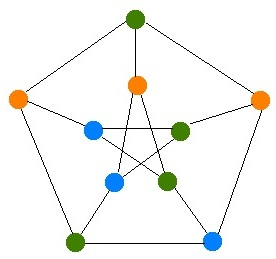
\includegraphics[scale=0.4]{seance8ex2}
     \end{center}
    \item  $\mathcal{X} = 2$ car ce graphe est biparti.
  \end{enumerate}
\end{solution}

\paragraph{3. } Vrai ou faux? \\
\begin{enumerate}[(a)]
  \item Un graphe de degré maximum 3 peut être colorié avec 4 couleurs.
  \item Un graphe de degré maximum 4 peut être colorié avec 4 couleurs.
  \item Si $G$ contient $K_n$ comme sous-graphe, alors son nombre chromatique est supérieur ou égal à $n$.
  \item Si $G$ est de nombre chromatique égal à $n$, alors $G$ contient $K_n$ comme sous-graphe.
\end{enumerate}

\begin{solution}
  \begin{enumerate}
    \item Vrai car $\mathcal{X} \leq$ degré max $+ 1 = 4$. 
    \item  Pas toujours. Le graphe $K_5$ en nécessite $5$ par exemple.
    \item Vrai puisqu'on aura déjà besoin de $5$ pour colorier $K_n$.
    \item Faux. Prenons par exemple un pentagone. Son nombre chromatique est égal à $3$ sans pour qu'il ne contienne de triangle. En fait, dès qu'on aura un cycle de longueur impaire, on va avoir $n \geq 3 $ sans pour autant que le graphe ne contienne $K_n$.
  \end{enumerate}
\end{solution}

\paragraph{4. } L'algorithme glouton de coloration associé à un graphe $G$ fonctionne comme suit: on parcourt les sommets $v_1,v_2,…,v_n$ de $G$ dans un ordre fixé arbitrairement. Lorsqu'on rencontre le sommet $v_i$, on lui assigne la plus petite couleur qui n'est pas encore utilisée par un de ses voisins.
\begin{enumerate}[(a)]
  \item Montrez que tout graphe $G$ possède une séquence de sommets pour laquelle l'algorithme glouton utilise un nombre minimum de couleurs.
  \item Construisez pour tout $k \geq 1$ un arbre de degré maximum $k$ et une séquence de ses sommets pour laquelle l'algorithme glouton utilise $k+1$ couleurs.
\end{enumerate}

\begin{solution}
  \begin{enumerate}
    \item En partant du graphe colorié, on peut créer une telle séquence en mettant d'abord tous les sommets de couleur $1$, puis tous les sommets de couleur $2$, etc. Le graphe obtenu à l'aide de l'algorithme glouton sera peut-être différent de celui qu'on avait au départ dans le sens où cet algorithme assigne la couleur la plus petite possible donc il se peut par exemple qu'il y a un noeud de couleur $2$ qui devienne de couleur $1$. L'algorithme glouton utilisera cependant bien le nombre minimal de couleurs, ce qui est bien ce qu'on veut!
    \item  Soit $A_1$ un noeud isolé. On peut ensuite créer $A_k$, avec $k \geq 2$, en créant un noeud relié à toutes les structures créées précédemment. La figure  ci-dessous illustre une telle construction.
    \begin{center}
    	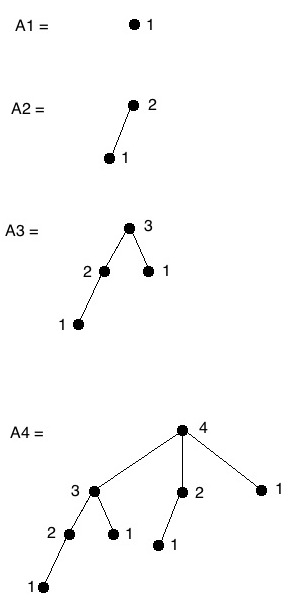
\includegraphics[scale=0.6]{seance8ex4}
     \end{center}
  \end{enumerate}
\end{solution}


\paragraph{5. } Pour les deux graphes ci-dessous appliquez l'algorithme de coloration glouton, et trouvez $\chi(G)$.


\begin{figure}[h!]
  \centering
  %\begin{center}
  \subfigure[]{
    \begin{tikzpicture}[-,>=stealth',shorten >=1pt,auto]
      \Vertex[x=0 ,y=0]{1}
      \Vertex[x=1 ,y=1]{2}
      \Vertex[x=2,y=0]{3}
      \Vertex[x=1 ,y=-1]{4}
      \Vertex[x=3 ,y=1]{5}
      \Vertex[x=3 ,y=-1]{6}
      \Vertex[x=4 ,y=0]{7}



      \path[every node/.style={font=\sffamily\small}]
      (1) edge node [left] {} (2)
      edge node [left] {} (5)
      edge node [left] {} (3)
      edge node [left] {} (4)
      edge node [left] {} (6)

      (2) edge node [right] {} (3)
      edge node [right] {} (7)
      edge node [right] {} (5)

      (3) edge node [right] {} (4)
      edge node [left] {} (5)
      edge node [left] {} (6)
      edge node [left] {} (7)

      (4) edge node [right] {} (6)
      edge node [right] {} (7)

      (5) edge node [right] {} (7)

      (6) edge node [right] {} (7);

  \end{tikzpicture} }
  \subfigure[]{
    \begin{tikzpicture}[-,>=stealth',shorten >=1pt,auto]
      \Vertex[x=0 ,y=0]{1}
      \Vertex[x=1 ,y=1]{2}
      \Vertex[x=1,y=0]{3}
      \Vertex[x=1 ,y=-1]{4}
      \Vertex[x=3 ,y=1]{5}
      \Vertex[x=3 ,y=-1]{6}
      \Vertex[x=2 ,y=0]{7}

      \path[every node/.style={font=\sffamily\small}]
      (1) edge node [left] {} (2)
      edge node [left] {} (3)
      edge node [left] {} (4)

      (2) edge node [right] {} (3)
      edge node [right] {} (7)
      edge node [right] {} (5)

      (3) edge node [right] {} (4)
      edge node [left] {} (7)

      (4) edge node [right] {} (6)
      edge node [right] {} (7)

      (5) edge node [right] {} (7)
      edge node [right] {} (6)

      (6) edge node [right] {} (7);

    \end{tikzpicture}
  }

\end{figure}

\begin{solution}
  \begin{enumerate}
    \item 
    \begin{itemize}
    \item noeud 1 $\Rightarrow$ couleur 1
    \item noeud 2 $\Rightarrow$ couleur 2
    \item noeud 3 $\Rightarrow$ couleur 3
    \item noeud 4 $\Rightarrow$ couleur 2
    \item noeud 5 $\Rightarrow$ couleur 4
    \item noeud 6 $\Rightarrow$ couleur 4
    \item noeud 7 $\Rightarrow$ couleur 1
    \end{itemize}
    Comme $K_4$ est inclus dans le graphe, on doit avoir $\mathcal{X} \geq 4$  et donc on a effectivement bien $\mathcal{X} = 4$.
    \item
    \begin{itemize}
    \item noeud 1 $\Rightarrow$ couleur 1
    \item noeud 2 $\Rightarrow$ couleur 2
    \item noeud 3 $\Rightarrow$ couleur 3
    \item noeud 4 $\Rightarrow$ couleur 2
    \item noeud 5 $\Rightarrow$ couleur 1
    \item noeud 6 $\Rightarrow$ couleur 3
    \item noeud 7 $\Rightarrow$ couleur 4
    \end{itemize}
    Regardons le cycle 23465. Puisqu'il est de longueur impaire, il va falloir 3 couleurs pour le colorier. Ensuite, on aura besoin d'une autre couleur pour le noeud $7$ comme il est relié à tous les noeuds du cycle. Dès lors, on a effectivement bien $\mathcal{X} = 4$ .
     \end{enumerate}
\end{solution}

\paragraph{6. } Sous quelle condition la somme des coefficients d'un polynôme chromatique est-elle nulle?
\begin{solution}
  La somme des coefficients du polynôme $= \pi_G(1)$ et $\pi_G(1) = 0$ veut dire que G a au moins une arête.
\end{solution}

\paragraph{7. } Trouvez le polynôme chromatique du graphe biparti complet $K_{2,2}$, et donnez le nombre de colorations possibles du cycle $C_4$ avec 5 couleurs.
\begin{solution}
  \begin{enumerate}
  \item En utilisant le fait que $\pi_k(G) = \pi_k(G-e) - \pi_k(G.e)$, on trouve que $\pi_k(K_{2,2}) = k^2(k-1)^2 - k (k-1)^2 - k(k-1)(k-2) = k^4-4k^3+6k^2-3k$.
  \item $C_4$ et $K_{2,2}$ sont isomorphes donc ils ont le même polynôme chromatique et $\pi_5(C_4) = \pi_5(K_{2,2}) = 5^4 - 4\cdot 5^3 + 6\cdot 5^2 - 3\cdot 5 = 260$.
\end{enumerate}
\end{solution}

\paragraph{8. }
\begin{enumerate}[(a)]
  \item Trouvez le polynôme chromatique d'un graphe chemin de longueur $n$
  \item Utilisez ce résultat pour trouver le polynôme chromatique d'un graphe circuit de longueur $n$.
\end{enumerate}
\begin{solution}
  \begin{enumerate}
  \item On démontre par récurrence que $p_k(P_n) = k(k-1)^n$.
  \item Etant donné que $\pi_k(G) = \pi_k(G-e) - \pi_k(G.e)$, on peut écrire que
           \begin{eqnarray*}
           p_k(C_n) &=& p_k(P_{n-1}) - p_k(C_{n-1})\\
           		    &=& k(k-1)^{n-1} - k(k-1)^{n-2} + ... + k(k-1)\\
		             &=& k(k-1) [(k-1)^{n-2} - (k-1)^{n-3} + ... + (-1)^n]\\
		             &=& k(k-1)\frac{1}{k}[(k-1)^{n-1}+(-1)^n]\\
		             &=& (k-1)^n + (-1)^n (k-1)
	   \end{eqnarray*}             
\end{enumerate}
\end{solution}

\paragraph{9. } Soit le graphe parallélépipède $3 \times 3 \times 2$.

\begin{enumerate}[(a)]
  \item Chaque arête du graphe est de longueur 1. On souhaite décrire un chemin qui part du sommet $s$ et arrive au sommet $t$ en passant au moins une fois par chaque arête. Quelle est la longueur minimale d'un tel chemin?
  \item Quel est le nombre minimum de couleurs nécessaires pour colorier les sommets de façon à ce que deux sommets adjacents soient toujours de couleurs différentes?
  \item Soit $P_G(k)$ le polynôme chromatique de ce graphe. Quel est le degré de $P_G(k)$? Que vaut $P_G(2)$?
  \item Trouvez une expression aussi explicite que possible pour le nombre de chemins de longueur $k$ du sommet $s$ à lui-même.
\end{enumerate}

\begin{figure}[h!]
  \centering
  %\includegraphics[scale=0.7]{img_tp8.jpg}
\end{figure}

\section{Graphes planaires}

% TODO Alexis, please merge BEGIN->MIDDLE and MIDDLE->END

% TODO BEGIN

Un graphe est planaire si il possède une représentation dans le plan dont les arêtes ne se touchent pas, sauf à leurs extrémités.\\

\begin{mytheo}[Conjoncture des quatre couleurs]
Quatre couleurs suffisent toujours pour colorier une carte
\begin{proof}
On suppose qu'en chaque point se rencontrent au maximum trois pays, et que les pays sont d'un seul tenant.\\

\begin{center}
\begin{tikzpicture}
%Outer box
\draw[fill=red] (-3,-3)--(-3,11)--(11,11)--(11,-3)--cycle;
%Outer circle
\draw (0,0) to[out=135,in=-135] (0,8);
\draw (0,8) to[out=45,in=135] (8,8);
\draw (8,8) to[out=-45,in=45] (8,0);
\draw (8,0) to[out=-135,in=-45] (0,0);

%First inner circle
\draw (1,4) to[out=90,in=-135] (2,6);
\draw (2,6) to[out=45,in=-180] (4,7);
\draw (4,7) to[out=0,in=135] (6,6);
\draw (6,6) to[out=-45,in=90] (7,4);
\draw (7,4) to[out=-90,in=45] (6,2);
\draw (6,2) to[out=-135,in=0] (4,1);
\draw (4,1) to[out=-180,in=-45] (2,2);
\draw (2,2) to[out=135,in=-90] (1,4);

%Second inner circle
\draw (3,4) to[out=90,in=-180] (4,5);
\draw (4,5) to[out=0,in=90] (5,4);
\draw (5,4) to[out=-90,in=0] (4,3);
\draw (4,3) to[out=-180,in=-90] (3,4);

%Links from Outer to first inner
\draw (0,0)--(2,2);
\draw (0,8)--(2,6);
\draw (8,8)--(6,6);
\draw (8,0)--(6,2);

%Links from first inner to second
\draw (1,4)--(3,4);
\draw (4,7)--(4,5);
\draw (7,4)--(5,4);
\draw (4,1)--(4,3);

%Regions
%1
\draw [fill = green](2,6) to[out=45,in=-180](4,7)to[out=0,in=135] (6,6)--(8,8)to[out=135,in=45](0,8)--(2,6);
\draw [fill= green](3,4) to[out=90,in=-180] (4,5)to[out=0,in=90](5,4) to[out=-90,in=0] (4,3)to[out=-180,in=-90] (3,4);
\draw[fill=green] (6,2) to[out=-135,in=0] (4,1)to[out=-180,in=-45] (2,2)--(0,0) to[out=-45,in=-135] (8,0)--(6,2);
%3
\draw [fill=yellow] (4,1) to[out=-180,in=-45] (2,2)to[out=135,in=-90] (1,4)--(3,4)to[out=-90,in=-180] (4,3)--(4,1);
\draw [fill=yellow] (4,7) to[out=0,in=135] (6,6)to[out=-45,in=90] (7,4)--(5,4)to[out=90,in=0] (4,5)--(4,7);
%4
\draw [fill=blue] (2,2) to[out=135,in=-90] (1,4)to[out=90,in=-135] (2,6)--(0,8)to[out=-135,in=135] (0,0)--(2,2);
\draw [fill=blue] (6,6) to[out=-45,in=90] (7,4)to[out=-90,in=45] (6,2)--(8,0)to[out=45,in=-45] (8,8)--(6,6);
\end{tikzpicture}
\end{center}

Il est possible de partir du graphe correspondant en remplacant les pays par des sommets et les frontières par des arêtes. Ce graphe est alors planaire. Il suffit alors de montrer que tout graphe planaire a un nombre chromatique $\chi \leq 4$ (ou de manière équivalente, admet au moins un coloriage de quatre couleurs).\\

Notons qu'un graphe planaire peut être dessiné de manière non planaire.
\end{proof}
\end{mytheo}
\begin{center}

\begin{tikzpicture}
\node[fill=black,  circle, inner sep=0pt,minimum width=0.5mm] (test) at (0,0) {\textbullet};
\node[fill=black,  circle, inner sep=0pt,minimum width=0.5mm] (test) at (0,4) {\textbullet};
\node[fill=black,  circle, inner sep=0pt,minimum width=0.5mm] (test) at (4,4) {\textbullet};
\node[fill=black,  circle, inner sep=0pt,minimum width=0.5mm] (test) at (4,0) {\textbullet};
\node[fill=black,  circle, inner sep=0pt,minimum width=0.5mm] (test) at (2,6) {\textbullet};
\node[fill=black,  circle, inner sep=0pt,minimum width=0.5mm] (test) at (1,2) {\textbullet};
\node[fill=black,  circle, inner sep=0pt,minimum width=0.5mm] (test) at (3,2) {\textbullet};

\draw (0,0)--(0,4)--(2,6)--(4,4)--(4,0)--cycle;
\draw (0,4)--(4,4);
\draw (0,0)--(1,2)--(2,6);
\draw (4,0)--(3,2)--(2,6);
\draw (0,4) to[out=-89, in=179] (4,0);
\end{tikzpicture}

\begin{tikzpicture}
\node[fill=black,  circle, inner sep=0pt,minimum width=0.5mm] (test) at (1,0) {\textbullet};
\node[fill=black,  circle, inner sep=0pt,minimum width=0.5mm] (test) at (1,4) {\textbullet};
\node[fill=black,  circle, inner sep=0pt,minimum width=0.5mm] (test) at (5,4) {\textbullet};
\node[fill=black,  circle, inner sep=0pt,minimum width=0.5mm] (test) at (5,0) {\textbullet};
\node[fill=black,  circle, inner sep=0pt,minimum width=0.5mm] (test) at (3,6) {\textbullet};
\node[fill=black,  circle, inner sep=0pt,minimum width=0.5mm] (test) at (0,2) {\textbullet};
\node[fill=black,  circle, inner sep=0pt,minimum width=0.5mm] (test) at (6,2) {\textbullet};
\draw (1,0)--(1,4)--(3,6)--(5,4)--(5,0)--cycle;
\draw (1,4)--(5,4);
\draw (1,0) to[out=135,in=-90](0,2)to[out=90,in=-150](3,6);
\draw (5,0) to[out=45,in=-90](6,2)to[out=90,in=-30](3,6);
\draw (1,4)--(5,0);
\end{tikzpicture}
\end{center}




\subsection{Graphes planaires}
\begin{mytheo} [Fáry]
Tout graphe planaire simple peut être représenté en n'utilisant que des arêtes droites.
%no proof ?
\end{mytheo}



\begin{mytheo}
Le graphe complet $K_5$ à cinq noeuds n'est pas planaire.

\begin{proof}

Représentons $K_5$ dans le plan. Soit l'ensemble de ses noeuds $\{v_1, v_2, v_3, v_4, v_5\}$.\\
$v_1, v_2$ et $v_3$ forment un triangle. Où placer $v_4$?

\begin{center}
\begin{tikzpicture}
\node[circle] (v1)[draw=black] at (0,0) {v1};
\node[circle] (v2)[draw=black] at (7,0) {v2};
\node[circle] (v3)[draw=black] at (2,5) {v3};
\draw (v1)--(v2)--(v3)--(v1);
\end{tikzpicture}
\end{center}


\begin{enumerate}
\item A l'intérieur du triangle formé par $v_1, v_2$ et $v_3$ ?\\
\begin{center}
\begin{tikzpicture}
\node[circle] (v1)[draw=black] at (0,0) {v1};
\node[circle] (v2)[draw=black] at (7,0) {v2};
\node[circle] (v3)[draw=black] at (2,5) {v3};
\node[circle] (v4)[draw=black] at (3,2) {v3};
\draw (v1)--(v2)--(v3)--(v1);
\draw (v4)--(v1);
\draw (v4)--(v2);
\draw (v4)--(v3);
\end{tikzpicture}
\end{center}
%\includegraphics[scale=0.4]{t2}\\
Où placer $v_5$?
\begin{enumerate}
\item A l'intérieur du triangle formé par $v_1, v_3$ et $v_4$ ? Le graphe ne serait plus planaire puisqu'il faudrait couper le triangle $v_1, v_3$ et $v_4$ pour relier $v_5$ à $v_2$.\\
\begin{center}
\begin{tikzpicture}
\node[circle] (v1)[draw=black] at (0,0) {v1};
\node[circle] (v2)[draw=black] at (7,0) {v2};
\node[circle] (v3)[draw=black] at (2,5) {v3};
\node[circle] (v4)[draw=black] at (3,2) {v3};
\node[circle] (v5)[draw=black] at (1.8,2.2) {v5};
\draw (v1)--(v2)--(v3)--(v1);
\draw (v4)--(v1);
\draw (v4)--(v2);
\draw (v4)--(v3);
\end{tikzpicture}
\end{center}
%\includegraphics[scale=0.4]{t3}
\item A l'intérieur de $v_1$, $v_2$, $v_4$ ou de $v_2$, $v_3$, $v_4$ ? Idem.
\item A l'extérieur de $v_1$, $v_2$, $v_3$? \\
\begin{center}
\begin{tikzpicture}
\node[circle] (v1)[draw=black] at (0,0) {v1};
\node[circle] (v2)[draw=black] at (7,0) {v2};
\node[circle] (v3)[draw=black] at (2,5) {v3};
\node[circle] (v4)[draw=black] at (3,2) {v3};
\node[circle] (v5)[draw=black] at (0,3) {v5};
\draw (v1)--(v2)--(v3)--(v1);
\draw (v4)--(v1);
\draw (v4)--(v2);
\draw (v4)--(v3);
\end{tikzpicture}
\end{center}
%\includegraphics[scale=0.4]{t4}\\
\end{enumerate}
\item A l'extérieur de $v_1, v_2$, $v_3$ ? En applicant le même type d'énumération qu'au point précédent, on trouve qu'il n'y a aucune manière de représenter $K_5$ dans le plan de manière à ce qu'il soit planaire.
\end{enumerate}
\end{proof}
\end{mytheo}



\begin{mytheo}
Le graphe complet biparti $K_{3,3}$ à $3+3$ noeuds n'est pas planaire.
\begin{proof}
Preuve \addTODO
\end{proof}
\end{mytheo}



\begin{mytheo} [Kuratowski]
  Un graphe est non planaire si et seulement s'il contient comme sous-graphe $K_5$ ou $K_{3,3}$ ou une subdivision de ceux-ci.
  \begin{proof}
    Preuve \addTODO
  \end{proof}
\end{mytheo}


\index{subdivision}
\begin{mydef}
  Une \emph{subdivision} (remplacement de chaque arête par un chemin) d'un graphe non planaire est non-planaire, et un sous-graphe d'un graphe planaire est planaire.
\end{mydef}

\index{face}
\index{face!face extérieure}
\index{face!face intérieure}
\begin{mydef}
  Un graphe planaire (dans une représentation sans croisement) découpe le plan en plusieurs régions connexes (au sens géométrique). Ces régions sont appelées \emph{faces}. Il y a une et une seule face non bornée, nommée \emph{face extérieure}, les autres faces sont \emph{intérieures}.
\end{mydef}

\index{face!bord d'une face}
\index{face!face incidente}
\index{face!degré d'une face}
\begin{mydef}
  On identifie le \emph{bord d'une face} au parcours fermé qui longe la face. Le bord parcourt chaque arête une ou deux fois. 
  Une face est \emph{incidente} aux arêtes et sommets qui sont sur son bord.
  Le \emph{degré d'une face} est la longueur du bord, donc le nombre d'arêtes incidentes (comptées une ou deux fois).
\end{mydef}
\begin{myexem}
  Exemple \addTODO
\end{myexem}

\index{dual}
\begin{mydef}
  Etant donné un graphe planaire $G$ (dans une représentation sans croisement), construisons $G^*$ , graphe dont les sommets sont les faces de $G$, reliés si et seulement si les faces correspondantes ont dans $G$ une arête en commun. Ce graphe $G^*$ est le \emph{dual} de $G$ (dans cette représentation).
\end{mydef}
\begin{myexem}

\noindent
\textit{Exemple} : \\
\begin{center}
\begin{tikzpicture}
%Premier graphe
\node[circle](N1)[draw=black] at (4,10) {1};
\node[circle](N2)[draw=black] at (4,8) {2};
\node[circle](N3)[draw=black] at (8,5) {3};
\node[circle](N4)[draw=black] at (4,2) {4};
\node[circle](N5)[draw=black] at (0,5) {5};
\node[circle](N6)[draw=black] at (2.5,5){6};

\draw (N1)--(N2)--(N3)--(N4)--(N5)--(N2);
\draw (N5)to[out=20,in=160](N6)to[out=-160,in=-20](N5);
\draw (N6)--(N2);

%Second graphe
\node (NN7) at (1.25,5) {\textbullet};
\node (NN8) at (2.5,6) {\textbullet};
\node (NN9) at (7,10) {\textbullet};
\node (NN10) at (6,5) {\textbullet};
\node [red] (test) at (8,11){Graphe Dual};
\node [black] (test) at  (7,2){Face exterieure};
\node [draw,text width =4cm] (test) at (13,8) 
{4 faces\\
Face extérieure : 1234521\\
degre(face exterieure=6)};

\coordinate (N7) at (1.25,5);
\coordinate (N8) at (2.5,6);
\coordinate (N9) at (7,10);
\coordinate (N10) at (6,5);

\draw[red] (N7) to[out=-20,in=-160](N10)--(N8)--(N7);
\draw[red] (N10)to[out=-160,in=90](1.5,2)to[out=-90,in=-180](4,0.5)to[out=0,in=-135](11,2.5)to[out=45,in=-30](N9)to[out=130,in=45](2,11)to[out=-135,in=135](N8);
\draw[red] (N10)to[out=-45,in=-135](8.5,4)to[out=45,in=-30](N9);
\draw[red] (N10)--(N9);
\draw[red] (N9) to[out=170,in=90](3,10)to[out=-90,in=-170](N9);

\end{tikzpicture}
\end{center}
\end{myexem}


\begin{mytheo}
  La somme des degrés des faces est deux fois le nombre d'arêtes.
  \begin{proof}
    Preuve \addTODO
  \end{proof}
\end{mytheo}

\begin{mytheo}
  Un graphe est planaire si et seulement si il est représentable sur la sphère sans croisement d'arêtes.
  \begin{proof}
    Preuve \addTODO
  \end{proof}
\end{mytheo}

%TODO END


\subsection{Formule d'Euler}
\begin{mytheo} [Formule d'Euler]
  Dans un graphe planaire connexe à $n$ sommets, $e$ arêtes et $f$ faces:\\
  $n−e+f =2$
  \begin{proof}
    On démontre cette égalité par récurrence sur sur le nombre d'arêtes. 
    	
    Si le graphe est sans cycle $\Rightarrow$ la face extérieure est la seule face. Le graphe est donc un arbre et on a donc 
    $$|arêtes|= |sommets|-1,$$ 
    $$|sommets| - |aretes| + |faces|= 2.$$	
    
  Si il existe un cycle, il y a donc deux faces adjacentes. En supprimant une arête entre les deux faces, les deux faces deviennent une seule et le nombre de faces moins le nombre d'arêtes reste constant. Par hypothèse de récurrence on a donc que  
  $$|sommets| - |aretes| + |faces|$$ 
  n'est pas modifié et vaut 2.
   
  \end{proof}
\end{mytheo}

\begin{mytheo}
  \label{theo:threensix}
  Dans tout graphe planaire \emph{simple} à $n \geq 3$ sommets et $e$ arêtes,
  $e \leq 3n - 6$.
  \begin{proof}
    Si il n'y a qu'une seule face, évident. 
    
    Si il y a au moins une face, le bord de la face a au moins 3 arêtes (vu que la plus petite face possible est un triangle et que c'est une graphe simple). On a donc deg(face)$\geq 3$. Et donc $$\sum \text{deg(face)} \geq 3 |faces| .$$
Or    $$\sum \text{deg(face)} = 2 |aretes|.$$
Et donc 
 \begin{equation} \label{ineg6}
 \frac{2}{3} |aretes| \geq |faces|.
\end{equation} 
    En injectant \ref{ineg6} dans la formule d'Euler, le résultat est démontré.   
  \end{proof}
\end{mytheo}

\begin{mytheo}
  Pour tout graphe planaire \emph{simple}, il y a un noeud de degré $\leq 5$.
  \begin{proof}
    On va montrer que le degré moyen est $< 6$.
    Ce qu'il voudra dire qu'il existe un noeud de degré $\leq 5$.
    \begin{align*}
      \deg_{\mathrm{avg}} & = \frac{\sum_{v\in V} \deg(v)}{|V|}\\
                          & = \frac{2|E|}{|V|}.
    \end{align*}
    Considérons 2 cas
    \begin{itemize}
      \item Si $|V| < 3$, l'énoncé est trivial car dans un graphe simple,
        pour tout $v \in V$, $\deg(v) \leq |V|-1$ du coup
        $\deg(v) \leq |V| - 1 < 2 \leq 5$ pour tout $v$.
      \item
        Comme notre graphe est simple,
        on peut utiliser le théorème~\ref{theo:threensix},
        on a donc $|E| \leq 3|V| - 6$.
        Dès lors
        \begin{align*}
          \deg_{\mathrm{avg}} & \leq 2\frac{3|V|-6}{|V|}\\
                              & = 6 - \frac{12}{|V|} < 6.
        \end{align*}
    \end{itemize}
  \end{proof}
\end{mytheo}

\begin{mycorr}
  $K_5$ est non planaire.
  \begin{proof}
    $K_5$ a 5 noeuds et 10 arêtes.
    Par le théorème~\ref{theo:threensix}, $|E| \leq 3|V| - 6$.
    Il faut donc que $10 \leq 3 \cdot 5 - 6 = 9$, ce qui est faux.
    Le graphe est par conséquent non planaire.
  \end{proof}
\end{mycorr}

\begin{mycorr}
  $K_{3,3}$ est non planaire.
  \begin{proof}
    $K_{3,3}$ a 6 noeuds et 9 arêtes.
    C'est un graphe biparti donc les cycles sont de longueur pair de plus il est simple donc tous les cycles ont une longueur $\geq 4$.
    Donc toutes les faces ont un degré $\geq 4$.
    On a alors $\sum_{f \in F} \deg(f) \geq 4|F|$ et par le théorème des poignées de main dual, $\sum_{f \in F} \deg(f) = 2|E| = 18$.
    Donc $|F| \leq \frac{18}{4} = 4.5$.

    Par la formule d'Euler, il faut que
    $|F| - |E| + |V| = 2$.
    Or $|F| - |E| + |V| \leq 4.5 - 9 + 6 = 1.5$.
    $K_{3,3}$ ne peut donc pas être planaire.
  \end{proof}
\end{mycorr}

\subsection{Les cinq solides platoniciens}
\index{solide platonicien}
\begin{mydef}
  Un \emph{solide platonicien} est un polyèdre convexe régulier.
  C'est-à-dire que toutes les faces, sommets et arêtes sont identiques à une rotation près.
\end{mydef}

\begin{mytheo}
  Il y a 5 solides platoniciens.
  \begin{proof}
    Les polyèdres convexes correspondent à des graphes planaires, via projection.
    Le fait qu'ils soient platoniciens nous dit que chaque noeud est de même degré $p$ et que chaque face est de même degré $q$.
    \begin{center}
      \begin{tabular}{ll}
        La formule d'Euler & $|F| - |E| + |V| = 2$\\
        Poignées de main & $p|V| = 2|E|$\\
        Poignées de main dual & $q|F| = 2|E|$
      \end{tabular}
    \end{center}
    Donc
    \begin{align*}
      \frac{2}{q}|E| - |E| + \frac{2}{p} |E| & = 2\\
      \frac{2}{q} - 1 + \frac{2}{p} & = \frac{2}{|E|} > 0\\
      \frac{1}{q} + \frac{1}{p} & > \frac{1}{2}.
    \end{align*}
    On sait donc que soit $p$, soit $q$ est $< 4$ (ou les deux).
    Or $p \geq 3$ et $q \geq 3$ (par géométrie, graphes planaires simple de dual simple).
    Les possibilités sont
    \begin{center}
      \begin{tabular}{|c|c|c|c|c|c|}
        \hline
        $p$ & $q$ & $|V|$ & $|F|$ & $|E|$ & Polyèdre\\
        \hline
         3  &  3  &   4   &   4   &   6   & Tétraèdre\\
         3  &  4  &   8   &   6   &  12   & Cube\\
         4  &  3  &   6   &   8   &  12   & Octaèdre\\
         3  &  5  &  20   &  12   &  30   & Dodécaèdre\\
         5  &  3  &  12   &  20   &  30   & Icosaèdre\\
        \hline
      \end{tabular}
    \end{center}
  \end{proof}
\end{mytheo}

\begin{mytheo} [Kempe]
  Tout graphe planaire possède un coloriage propre à cinq couleurs.
  ``Toute carte peut être coloriée avec 5 couleurs''.\\
  Nombre chromatique $\chi$ (graphe planaire) $\leq 5$.
  \begin{proof}
    Par récurrence: ``on enlève un noeud, on colorie par hyp. de récurrence, on remet le noeud.''
    On peut supposer le graphe \emph{simple} (car arêtesmultiples n'affectent pas $\chi$).
    Il existe un noeud $u$ de degré $\leq 5$.
    On enlève $u$, on a encore un graphe planaire, on le colorie.
    On rétablit $u$:
    \begin{itemize}
      \item si $\deg(u) < 5$: facile, on utilise une couleur non utilisée par les voisins pour $u$.
      \item Si $\deg(u) = 5$: Si ces 5 voisins utilisent $< 5$ couleurs: facile aussi.
        Si 5 couleurs utilisées $c_1, c_2, c_3, c_4, c_5$.
        Regardons $v_1$ et $v_3$. Si $v_1$ et $v_3$ sont sur des composantes connexes différentes: on échange $c_1$ et $c_3$ sur
        la composante connexe ($c_1-c_3$) de $v_3$, et on colorie $u$ en $c_1$ (sur le graphe des noeuds de couleur $c_1$ et $c_3$.
        Si $v_1$ et $v_3$ sont dans la même composante connexe ($c_1-c_3$):
        Maintenant $v_2$ et $v_4$ sont dans des composantes connexes
        différentes (dans le graphe de couleurs $c_2-c_4$).
        Même raisonnement: échanger $c_2$ et $c_4$ sur composante connexe ($v_2$).
    \end{itemize}
  \end{proof}
\end{mytheo}

\begin{mytheo} [Appel, Haken]
  Tout graphe planaire possède un coloriage propre à quatre couleurs.
  \begin{proof}
    Preuve \addTODO
  \end{proof}
\end{mytheo}

\section{Flots et coupes}
\subsection{Flots et coupes}
\index{flot}
\index{capacité}
\begin{mydef}
  Soit un graphe dirigé, dont les noeuds sont partitionnés en sources, puits et noeuds intermédiaires, et dont chaque arête $a$ porte un nombre réel $c(a)$ nommé \emph{capacité}.\\
  Un \emph{flot} est la donnée d'un nombre réel $f(a)$ sur chaque arête, tel que $0 \leq f(a) \leq c(a)$ et que le flot net sortant de chaque noeud intermédiaire soit nul.
\end{mydef}

\index{flot!flot net sortant}
\index{flot!valeur du flot}
\index{flot!flot maximum}
\begin{mydef}
  \begin{itemize}
    \item Le \emph{flot net sortant d'un noeud} $u$ est défini comme
      $\sum_{\text{arêtes }a\text{ d'origine }u} f(a) − \sum_{\text{arêtes }b\text{ de destination }u} f(b)$.
    \item Le \emph{flot net sortant d'un ensemble} $U$ de noeuds est la somme des flots nets sortant des noeuds de $U$.
    \item La \emph{valeur du flot} est le flot net sortant des noeuds sources.
  \end{itemize}
  On désire trouver le \emph{flot maximum}, c'est-à-dire le flot de valeur maximale.
\end{mydef}

\index{coupe}
\index{coupe!coupe minimum}
\begin{mydef}
  Une \emph{coupe} est un ensemble d'arêtes tel qu'il n'ait plus aucun chemin d'un noeud source vers un noeud puits quand on retire cet ensemble du graphe.\\
  On désire trouver une \emph{coupe minimum}, c'est-à-dire une coupe dont la capacité (i.e., la somme des capacités de ses arêtes) est minimale.
\end{mydef}

\begin{center}
  \begin{tikzpicture}
    \node[vertex] at (0, 0) (s) {\tiny $s$};
    \node[vertex] at (2, 1) (a) {\tiny $a$};
    \node[vertex] at (2, -1) (b) {\tiny $b$};
    \node[vertex] at (4, 1) (c) {\tiny $c$};
    \node[vertex] at (4, -1) (d) {\tiny $d$};
    \node[vertex] at (6, 0) (t) {\tiny $t$};
    \draw[->] (s) edge node[anchor = south] {\tiny $0 / 3$} (a);
    \draw[->] (s) edge node[anchor = north] {\tiny $0 / 2$} (b);
    \draw[->] (a) edge node[anchor = south] {\tiny $0 / 2$} (c);
    \draw[->] (a) edge node[anchor = south] {\tiny $0 / 3$} (d);
    \draw[->] (b) edge node[anchor = north] {\tiny $0 / 2$} (d);
    \draw[->] (c) edge node[anchor = south] {\tiny $0 / 2$} (t);
    \draw[->] (d) edge node[anchor = north] {\tiny $0 / 2$} (t);
  \end{tikzpicture}
\end{center}

\begin{center}
  \begin{tikzpicture}
    \node[draw, circle] at (-2,0) (S) {S};
    \node[draw, circle] at (-1,1) (A) {};
    \node[draw, circle] at (-1,-1) (B) {};
    \node[draw, circle] at (1,1) (C) {};
    \node[draw, circle] at (1,-1) (D) {};
    \node[draw, circle] at (2,0) (P) {P};

    \draw[->] (S) edge node[anchor = south] {$3/6$} (A);
    \draw[->] (S) edge node[anchor = south] {$1/4$} (B);
    \draw[->] (A) edge node[anchor = south] {$2/4$} (C);
    \draw[->] (A) edge node[anchor = south] {$1/1$} (D);
    \draw[->] (B) edge node[anchor = north] {$1/1$} (C);
    \draw[->] (B) edge node[anchor = north] {$2/2$} (D);
    \draw[->] (C) edge node[anchor = south] {$1/3$} (P);
    \draw[->] (D) edge node[anchor = south] {$3/3$} (P);
  \end{tikzpicture}
\end{center}

\paragraph{Observation}
Se donner une coupe, on se donne un ensemble $S$ de noeuds atteignables à partir des sources,
c'est la même chose.
Lorsqu'on a une coupe, $S$ est la composante connexe comprenant les sources lorsqu'on enlève la coupe.
Lorsqu'on a $S$, la coupe est l'ensemble des arêtes reliant un noeud de $S$ et de $\bar{S}$.

\begin{mylem}
  Pour un flot donné, toutes les coupes ont le même flot net, qui est la valeur du flot.
  \begin{proof}
    Flot net de la coupe = Flot net(sources) + Flot net (s$\setminus$sources)
    =$f(S \to \bar{S}) - f(\bar{S} \to S)$
    taille de la coupe = capacité totale de la coupe
    \begin{center}
      \begin{tikzpicture}
        \node[draw, circle] at (-2,0) (S1) {S};
        \node[draw, circle] at (-2,-1) (S2) {S};
        \node[draw, circle] at (-1,1) (A1) {};
        \node[draw, circle] at (-1,0) (A2) {};
        \node[draw, circle] at (-1,-1) (A3) {};
        \node[draw, circle] at (0,2) (B1) {};
        \node[draw, circle] at (0,1) (B2) {};
        \node[draw, circle] at (0,0) (B3) {};
        \node[draw, circle] at (0,-1) (B4) {};
        \node[draw, circle] at (1,2) (P1) {P};
        \node[draw, circle] at (1,1) (P2) {P};
        \node[draw, circle] at (1,0) (P3) {P};
        \node[draw, circle] at (1,-1) (P4) {P};

        \draw[->] (S1) edge (A1);
        \draw[->] (S1) edge (A2);
        \draw[->] (S1) edge (A3);
        \draw[->] (S2) edge (A3);
        \draw[->] (A1) edge (B1);
        \draw[->] (A1) edge (B2);
        \draw[->] (A2) edge (B2);
        \draw[->] (A2) edge (B3);
        \draw[->] (A3) edge (B4);
        \draw[->] (B1) edge (P1);
        \draw[->] (B2) edge (P2);
        \draw[->] (B3) edge (P3);
        \draw[->] (B4) edge (P4);
      \end{tikzpicture}
    \end{center}
  \end{proof}
\end{mylem}

\begin{mylem}
  Pour tout flot $f$ et toute coupe $S \to \bar{S}$,
  $\valeur(f) \leq \coupe(S \to \bar{S})$.
  L'égalité a lieu si et seulement si toutes les arêtes $a$ de la coupe $S \to \bar{S}$ sont $f$-saturées
  (i.e., $f(a) = c(a)$) et toutes les arêtes $b$ de $\bar{S} \to S$ sont $f$-nulles (i.e., $f(b) = 0$).

  \begin{proof}
    \begin{align*}
      \valeur(f) & = \text{flot sur la coupe}\\
             & = \sum \fnet(S \to \bar{S})\\
             & = \sum_{i \in S \atop {j \in \bar{S} \atop ij \in E}} f(ij) - \sum_{i \in S \atop {j \in \bar{S} \atop ji \in E}} f(ij)\\
             & \leq \sum_{i \in S \atop {j \in \bar{S} \atop ij \in E}} f(ij)\\
             & \leq \sum_{i \in S \atop {j \in \bar{S} \atop ij \in E}} c(ij)\\
             & = \coupe(S \to \bar{S}).
    \end{align*}
    Avec égalité si et seulement si $\sum_{i \in S\atop {j \in \bar{S}\atop ji \in E}} f(ij) = 0$ et
    $\sum_{i \in S\atop {j \in \bar{S}\atop ij \in E}} f(ij) = \sum_{i \in S\atop {j \in \bar{S}\atop ij \in E}} c(ij)$
    c'est à dire que toutes les arêtes qui lient un noeud de $S$ à un noeud de $\bar{S}$ sont saturées
    et que les arêtes qui lient un noeud de $\bar{S}$ à un noeud de $S$ ont un flot nul.
  \end{proof}
\end{mylem}

\begin{mycorr}
  Si un flot $f$ et une coupe $S\to\bar{S}$ sont tels que $\valeur(f) = \coupe(S\to\bar{S})$,
  alors ce flot est maximum et cette coupe minimum.
  \begin{proof}
    On vient de voir que dans le cas d'égalité, les arêtes étaient saturées et il n'y a aucun flot qui va de $\bar{S}$ à $S$
    Et donc ne peut plus faire passer de flot de $S$ à $\bar{S}$ ni par des arêtes directes (elles sont saturées),
    ni par des ``back edges'' (elles sont nulles car il n'y a pas de flot de $\bar{S}$ à $S$).

    Le fait que le flot est maximum et que la coupe est minimum est en fait simplement montré par la dualité.
    On sait que pour toute coupe $S\to\bar{S}$ et flot $f$, $\coupe(S\to\bar{S}) \geq \valeur(f)$.
    Dès lors, pour toute coupe $\coupe(S \to \bar{S}) \geq \flotmax$ et pour tout flot,
    $\coupemin \geq \valeur(f)$ et en particulier
    $\coupemin \geq \flotmax$.
    On a donc
    \[ \coupe(S \to \bar{S}) \geq \coupemin \geq \flotmax \geq \valeur(f) \]
    d'où $\coupe(S \to \bar{S}) = \coupemin$ et
    $\flotmax = \valeur(f)$ en cas d'égalité
    $\coupe(S \to \bar{S}) = \valeur(f)$.
  \end{proof}
\end{mycorr}

\index{chemin!chemin $f$-saturé}
\index{chemin!chemin $f$-augmentant}
\begin{mydef}
  Etant donné un flot $f$, à tout chemin $P$ dans le graphe non-dirigé sous-jacent associons la quantité $i(P) = \min_{a \in P} i(a)$, où $i(a) = c(a) − f(a)$ pour les arêtes $a$ prises par $P$ dans le sens direct, et $i(a) = f (a)$ pour les arêtes a prises dans le sens inverse.\\
  Un chemin $P$ est \emph{$f$-saturé} si $i(P) = 0$. Il est \emph{$f$-augmentant} s'il est non saturé, part d'un noeud source et arrive à un noeud puits.
\end{mydef}

\begin{myexem}
  En partant du flot $f$ avec un chemin $f$-augmentant
  montré à la figure~\ref{fig:faug},
  on peut créer un nouveau flot $f'$ valide.
  L'arête déjà remplie à $3/4$ nous oblige à ce que le flot n'augmente que de 1,
  $\valeur(f') = \valeur(f) + 1$.
  Le flot est alors modifié le long de ce chemin comme montré
  à la figure~\ref{fig:fprime}.
  \begin{figure}[h!]
    \centering
    \begin{tikzpicture}
      \SetGraphUnit{2}
      \GraphInit[vstyle=Dijkstra]
      \SetUpEdge[style={->},
      labelstyle = {draw}]
      \Vertex{S}
      \NOEA(S){A}
      \SOEA(A){B}
      \NOEA(B){C}
      \SOEA(C){D}
      \NOEA(D){T}
      \Edge[label=$1/5$](S)(A)
      \Edge[label=$2/3$](B)(A)
      \Edge[label=$3/4$](B)(C)
      \Edge[label=$2/2$](D)(C)
      \Edge[label=$0/4$](D)(T)
    \end{tikzpicture}
    \caption{Chemin $f$-augmentant}
    \label{fig:faug}
  \end{figure}
  \begin{figure}[h!]
    \centering
    \begin{tikzpicture}
      \SetGraphUnit{2}
      \GraphInit[vstyle=Dijkstra]
      \SetUpEdge[style={->},
      labelstyle = {draw}]
      \Vertex{S}
      \NOEA(S){A}
      \SOEA(A){B}
      \NOEA(B){C}
      \SOEA(C){D}
      \NOEA(D){T}
      \Edge[label=$2/5$](S)(A)
      \Edge[label=$1/3$](B)(A)
      \Edge[label=$4/4$](B)(C)
      \Edge[label=$1/2$](D)(C)
      \Edge[label=$1/4$](D)(T)
    \end{tikzpicture}
    \caption{Chemin avec $f'$}
    \label{fig:fprime}
  \end{figure}
\end{myexem}

\begin{mytheo}
  Un flot est maximum si et seulement s'il ne contient pas de chemin $f$-augmentant.
  \begin{proof}
    \begin{itemize}
      \item[$\Rightarrow$] Si il existe un chemin augmentant, alors on peut améliorer strictement le flot.
      \item[$\Leftarrow$]
        Soit $f$ un flot qui ne contient pas de chemin $f$-augmentant.
        Soit $S$ l'ensemble des noeuds qu'on peut atteindre à partir de la source avec
        des chemins non $f$-saturés.
        $S$ ne contient aucun puits.
        Soit une arête de $S \to \bar{S}$, elle est $f$-saturée par construction de $S$,
        sinon la destination de l'arête serait dans $S$.
        Soit une arête de $\bar{S} \to S$, elle doit être $f$-nulle pour la même raison.
        \begin{figure}[h!]
          \centering
          \begin{tikzpicture}[x=2cm,y=1cm]
            \SetGraphUnit{1}
            \GraphInit[vstyle=Dijkstra]
            \SetUpEdge[style={->},
            labelstyle = {draw}]
            \Vertex{S}
            \NOEA(S){A}
            \SOEA(S){B}
            \EA(A){a}
            \EA(B){b}
            \SOEA(a){T}
            \Edge[label=$4/4$,color=red](A)(a)
            \Edge[label=$0/5$,color=red](b)(B)
            \AddVertexColor{blue}{S,A,B}
            \AddVertexColor{green}{a,b,T}
          \end{tikzpicture}
        \end{figure}
        Dès lors,
        \begin{align*}
          \coupe(S\to\bar{S}) & = \text{valeur du flot qui quitte }S\text{ vers }\bar{S}\\
                              & = \text{valeur du flot net entre }S\text{ et }\bar{S}\\
                              & = \valeur(f)
        \end{align*}
        Cette coupe est la coupe mininum et ce flot est le flot maximum.
        La preuve prouve aussi que du flot max on déduit une coupe min de même valeur.\\ D'où  $\rightarrow$ Max Flow = Min cut.
    \end{itemize}
  \end{proof}
\end{mytheo}

\begin{mytheo}
  La valeur du flot maximum et la capacité de la coupe minimum sont toujours égales.
  \begin{proof}
    Cette preuve n'a pas été vue au cours, on l'obtiens cependant facilement par contradiction.
  \end{proof}
\end{mytheo}

\subsection{L'algorithme de Ford-Fulkerson}
\index{algorithme!algorithme de Ford-Fulkerson}
\begin{myalgo}[Algorithme de Ford-Fulkerson]
  L'algorithme a été vu au cours du dernier APE.
\end{myalgo}


\begin{mylem}
  \label{lem:flot_chemin}
  Dans tout graphe dirigé avec un noeud source $u$ et un noeud puits $v$ et chaque arête de capacité un, le nombre maximum de chemins dirigés de u vers v disjoints deux à deux par les arêtes est la valeur du flot maximum.
  \begin{proof}
    Si j'ai $k$ chemins disjoints $u \to v$,
    je crée un flot de valeur $k$ en saturant les arêtes
    des chemins.
    \begin{figure}[h!]
      \centering
      \begin{tikzpicture}
        \SetGraphUnit{2}
        \GraphInit[vstyle=Dijkstra]
        \SetUpEdge[style={->},
        labelstyle = {draw}]
        \Vertex{S}
        \NOEA(S){A1}
        \EA(A1){A2}
        \SOEA(A2){T}
        \EA(S){B1}
        \EA(B1){B2}
        \EA(B2){T}
        \SOEA(S){C1}
        \EA(C1){C2}
        \NOEA(C2){T}
        \Edge[label=$1/1$](S)(A1)
        \Edge[label=$1/1$](A1)(A2)
        \Edge[label=$1/1$](A2)(T)
        \Edge[label=$1/1$](S)(B1)
        \Edge[label=$1/1$](B1)(B2)
        \Edge[label=$1/1$](B2)(T)
        \Edge[label=$1/1$](S)(C1)
        \Edge[label=$1/1$](C1)(C2)
        \Edge[label=$1/1$](C2)(T)
      \end{tikzpicture}
    \end{figure}
    $\flotmax \geq \#\{\text{chemins disjoints }u \to v\}$.

    De plus, considérons le flot max de $u \to v$.
    Partant d'un flot initial \emph{entier},
    Ford-Fulkerson le maintient \emph{entier},
    d'où il existe un flot maximum entier.

    Il existe donc un flot maximum binaire: 0 ou 1
    sur chaque arête.
    Prenons $E$, le nombre d'arêtes de flot 1.
    C'est un sous-graphe.
    Si ni source ni puits,
    degré entrant = degré sortant (sur $E$).
    Si $\flotmax = k$,
    il existe $k$ arêtes sortantes de $u$ dans $E$ que
    je peux prolonger par $k$ chemins (disjoints par les arêtes)
    vers $v$.

    \begin{figure}[h!]
      \centering
      \begin{tikzpicture}[x=2cm,y=1cm]
        \SetGraphUnit{1}
        \GraphInit[vstyle=Dijkstra]
        \SetUpEdge[style={->},
        labelstyle = {draw}]
        \SetVertexNoLabel
        \Vertex[NoLabel=false,L=$u$]{u}
        \NOEA(u){a}
        \SOEA(u){b}
        \SOEA(a){o}
        \NOEA(o){c}
        \SOEA(o){d}
        \SOEA[NoLabel=false,L=$v$](c){v}
        \Edges[color=blue](u,a,o,d,v)
        \Edges[color=green](u,b,o,c,v)
      \end{tikzpicture}
    \end{figure}
  \end{proof}
\end{mylem}

\begin{mytheo}
  \label{theo:kconnexe_chemin}
  Un graphe (non-dirigé) est $k$-arête-connexe si et seulement si entre toutes paires de noeuds il y a au moins $k$ chemins disjoints deux à deux par les arêtes.
  \begin{proof}
    \begin{itemize}
      \item[$\Leftarrow$]
        Si j'enlève $k-1$ arêtes quelconques
        entre $u$ et $v$, je coupe au plus $k-1$
        chemins des $k$ chemins disjoints.
        Il en reste au moins 1.
      \item[$\Rightarrow$]
        $k$-arête-connexe signifie que toute coupe entre $u$
        et $v$ a une capacité d'au moins $k$ (pour capacité 1
        sur les arêtes) car $\coupemin = k$.
        Le flot max de $u$ vers $v$ est donc $k$.
        Par le Lemme~\ref{lem:flot_chemin},
        il existe $k$ chemins disjoints par les arêtes de
        $u \to v$.
    \end{itemize}
  \end{proof}
\end{mytheo}

\begin{mytheo} [Menger]
  Un graphe (non-dirigé) est $k$-connexe si et seulement si entre chaque paire de noeuds il y a au moins $k$ chemins disjoints deux à deux par les noeuds.
  \begin{proof}
    Pour se ramener au théorème~\ref{theo:kconnexe_chemin},
    on va ``tranformer les noeuds en arêtes''.
    \begin{table}[h!]
      \centering
      \begin{tabular}{cc}
        Graphe non dirigé $G$ & Graphe dirigé $G'$\\
        \begin{tikzpicture}
          \SetGraphUnit{1}
          \GraphInit[vstyle=Dijkstra]
          \SetUpEdge[style={->}]
          \Vertex[L=$u$]{u}
        \end{tikzpicture}
        &
        \begin{tikzpicture}
          \SetGraphUnit{1}
          \GraphInit[vstyle=Dijkstra]
          \SetUpEdge[style={->}]
          \Vertex[L=$u_0$]{u0}
          \EA[L=$u_1$](u0){u1}
          \Edge(u0)(u1)
        \end{tikzpicture}\\
        \begin{tikzpicture}
          \SetGraphUnit{1}
          \GraphInit[vstyle=Dijkstra]
          \Vertex[L=$u$]{u}
          \SO[L=$v$](u){v}
          \Edge(u)(v)
        \end{tikzpicture}
        &
        \begin{tikzpicture}
          \SetGraphUnit{1}
          \GraphInit[vstyle=Dijkstra]
          \SetUpEdge[style={->}]
          \Vertex[L=$u_0$]{u0}
          \EA[L=$u_1$](u0){u1}
          \SO[L=$v_0$](u0){v0}
          \EA[L=$v_1$](v0){v1}
          \Edge(u0)(u1)
          \Edge(v0)(v1)
          \Edge(u1)(v0)
          \Edge(v1)(u0)
        \end{tikzpicture}\\
        \begin{tikzpicture}
          \SetGraphUnit{1}
          \GraphInit[vstyle=Dijkstra]
          \Vertex[L=$u$]{u}
          \SO[L=$v$](u){v}
          \SO[L=$w$](v){w}
          \Edge(u)(v)
          \Edge(v)(w)
        \end{tikzpicture}
        &
        \begin{tikzpicture}
          \SetGraphUnit{1}
          \GraphInit[vstyle=Dijkstra]
          \SetUpEdge[style={->}]
          \Vertex[L=$u_0$]{u0}
          \EA[L=$u_1$](u0){u1}
          \SO[L=$v_0$](u0){v0}
          \EA[L=$v_1$](v0){v1}
          \SO[L=$w_0$](v0){w0}
          \EA[L=$w_1$](w0){w1}
          \Edge(u0)(u1)
          \Edge(v0)(v1)
          \Edge(w0)(w1)
          \Edge(u1)(v0)
          \Edge(v1)(u0)
          \Edge(v1)(w0)
          \Edge(w1)(v0)
        \end{tikzpicture}\\
      \end{tabular}
    \end{table}[h!]
    $k$ chemins $u \to v$ disjoints par les noeuds
    $\rightarrow$ en $k$ chemins $u_0 \to v_1$ disjoints
    par les arêtes.
    Flot max $u \to v$ $\rightarrow$ Flot max de $u_0 \to v_1$
    de même valeur.

    $k$-connexe $\leftrightarrow$ en $k$-arête connexe.
    On applique le théorème~\ref{theo:kconnexe_chemin} sur $v'$,
    on en déduit le théorème de Menger sur $v$.
  \end{proof}
\end{mytheo}



\end{document}
